% =====================================================================
%  Aegis -- Final Evaluation Report (UCS503P, TIET)
%  Built on the TIET report class (tietreport.cls, v1.0.4).
%  Compile on Overleaf with pdfLaTeX; the bibliography uses biblatex +
%  Biber, which Overleaf runs automatically.
% =====================================================================
\documentclass{tietreport}

% Import images (also loaded by the class)
\usepackage{graphicx}

% ---------- Extra packages used by this report ----------
\usepackage[T1]{fontenc}
\usepackage[utf8]{inputenc}
\usepackage{float}
\usepackage{placeins}
\usepackage{rotating}
\usepackage{array,tabularx}
\usepackage{enumitem}
\usepackage{caption}
\usepackage{xcolor}
\usepackage{algorithm}
\usepackage{algpseudocode}
\usepackage{tikz}
\usetikzlibrary{arrows.meta,positioning}
\usepackage{csquotes}
\usepackage{xurl}

% Bibliography configuration (as in the template)
\usepackage[
  date=year,
  style=alphabetic,
  backend=biber,
  sorting=nty,
  maxnames=5,
  minnames=3,
  maxalphanames=4,
  minalphanames=3,
  backref=true,
  doi=false,
  isbn=false,
  url=false,
  eprint=false
]{biblatex}
\addbibresource{references.bib}

\graphicspath{{figures/}}

%% ==================================================
%% PROJECT FIELDS
%% ==================================================

% Course/Lab header
\TitlePageHeader{%
  UCS503P -- Software Engineering (Laboratory)%
}

% Main project title
\ProjectTitle{%
  Aegis%
}

% Subtitle or project description
\ProjectSubTitle{%
  An Encrypted Dead-Man's-Switch Legacy Vault using Shamir's Secret Sharing%
}

% Student information
\author{%
  \texttt{1024030001} Pratham Arora \\
  \texttt{1024030009} Krishna Pandey \\
  \texttt{1024030881} Nipun Behl%
}

% Group number, degree, year, program
\TitlePageSubText{%
  Group: \texttt{3C11} BE Third Year, COE%
}

% Faculty advisor/guide name
\AdvisorName{%
  Dr.\ Paramveer Sidhu%
}

% Evaluation period and department info
\TitlePageFooterText{{%
    \large Final Evaluation \\[0.2cm]
    \bfseries Computer Science and Engineering
    Department%
  } \\[0.15cm]
  Thapar Institute of Engineering and Technology,
  Patiala \\[0.1cm]
  {\small 2026--27 ODD Semester}%
}

%% ==================================================

% ---------- Helpers ----------
\newcommand{\req}[1]{\texttt{#1}}          % requirement / threat IDs, e.g. \req{FR-4}
\newcommand{\code}[1]{\texttt{#1}}         % file names, functions, endpoints
\captionsetup{font=small,labelfont=bf}
\setlist{itemsep=2pt}
\setlength{\emergencystretch}{3em}
\renewcommand{\arraystretch}{1.2}
\newcolumntype{L}[1]{>{\raggedright\arraybackslash}p{#1}}
\newcolumntype{Y}{>{\raggedright\arraybackslash}X}

\hypersetup{
  pdftitle={Aegis: An Encrypted Dead-Man's-Switch Legacy Vault},
  pdfauthor={Pratham Arora, Krishna Pandey, Nipun Behl},
  pdfsubject={UCS503P -- Software Engineering (Laboratory): Final Evaluation Report}
}

\begin{document}

% Generate title page
\maketitle

% Table of contents (auto-generated from chapters)
\tableofcontents

% ===== CHAPTER 1: INTRODUCTION =====

\chapter{Introduction}\label{ch:introduction}

\section{Background and Context}\label{sec:intro-background}

A growing share of what people own and know now exists only in digital form:
banking and brokerage credentials, cryptocurrency keys, password-manager master
passwords, encrypted archives, business-continuity information and personal
messages meant for particular people. The value of this material is entirely
conditional on access, and access is exactly what is lost when its owner dies
or becomes permanently incapacitated. Unlike a physical estate, a forgotten
password or an unrecorded key cannot be recovered by an executor; the data
simply becomes unreachable.

Existing approaches force an uncomfortable choice. Sharing passwords with a
relative or friend makes the secret readable from the moment it is shared, and
its safety then depends indefinitely on the honesty, competence and
availability of one person. Appointing a single executor or custodian
concentrates the same risk in one party and is triggered by a slow legal
process rather than by the owner's absence. Provider-held recovery schemes, in
which a service keeps the means to unlock an account, require trusting the
provider and anyone who compromises it with the plaintext. In every case there
is a single point of failure: one document, one person or one operator whose
loss, compromise or delay defeats the owner's intent.

The project therefore combines two ideas. A \emph{dead man's switch} releases
information when its owner stops responding, so the trigger is the owner's
sustained silence rather than a human decision. \emph{Threshold secret
sharing}~\cite{shamir1979} removes the single custodian: the decryption key is
split among several trustees so that any $K$ of $N$ of them can rebuild it,
while any $K-1$ learn nothing at all. Aegis adds a third property that recent
breaches have made essential: the service that runs the switch should never be
able to read what it protects.

\subsection{Problem Statement}\label{sec:intro-problem}

The problem addressed is how to release a secret to designated recipients
when, and only when, its owner has become unresponsive, without any single
party --- including the system operator --- being able to read the secret
beforehand, and without depending on any single custodian. The scope is fixed
by the SRS: one vault per owner (\req{NG-3}); check-in prompts and release
notices by email only, with no SMS (\req{NG-1}) and no native mobile
application (\req{NG-2}); $N$ trustees with a reconstruction threshold of at
least two (\req{FR-4}); and a zero-knowledge server that stores only
ciphertext and trustee-encrypted shares (\req{NFR-SEC-5}). The catastrophic
failure mode is premature release, which is irreversible (\req{NFR-REL-1}).

\subsection{Scope of this Report}\label{sec:intro-scope}

This report describes the final product submitted for the end-semester
evaluation. It extends the prototype report with the work done since the
prototype evaluation --- the live production deployment, a redesigned user
interface with light and dark themes, accessibility and search-engine fixes,
dependency maintenance and the tooling used to prepare live demonstrations
(Section~\ref{sec:design-final}) --- and repeats the measurements on the
final build (Chapter~\ref{ch:results}). The product is live at
\url{https://ucs503p-aegis.vercel.app} and its source code, tests and
measurement scripts are in the repository
\url{https://github.com/Pratham-90/ucs503p-aegis}.

\section{Project Objectives}\label{sec:intro-objectives}

\begin{enumerate}
  \item \textbf{Objective 1:} Never release a vault before its deadline plus
    grace period: zero early releases across at least 1,000 simulated
    schedules with injected faults (\req{NFR-REL-1}, \req{NFR-REL-3}).
  \item \textbf{Objective 2:} Keep the server zero-knowledge: an automated
    inspection of everything the server stores and receives finds no plaintext
    payload, key or share (\req{FR-2}, \req{FR-2a}, \req{NFR-SEC-1},
    \req{NFR-SEC-5}).
  \item \textbf{Objective 3:} Make the threshold property demonstrable and
    verified: any $K$ of $N$ shares recover the vault, fewer than $K$ fail,
    verified by property-based tests and an end-to-end browser test of the full
    demo script (\req{FR-8}, \req{NFR-SEC-2}).
  \item \textbf{Objective 4:} Implement the cryptographic core twice --- an
    authoritative Python implementation and the deployed TypeScript client ---
    and bind them with shared known-answer test vectors that agree on every
    case (\req{FR-2a}).
  \item \textbf{Objective 5:} Keep check-ins fast and the code maintainable:
    check-in confirmation p95 within 500\,ms under nominal load
    (\req{NFR-PERF-1}) and at least 80\% test coverage on the crypto and
    scheduler packages (\req{NFR-MAINT-1}), on a live deployment (Vercel with
    Neon Postgres).
\end{enumerate}

These are SMART objectives (Specific, Measurable, Achievable, Relevant,
Time-bound), each tied to SRS requirements. Objectives 1--4 were due at the
prototype milestone (Week~8 of the 12-week plan) and Objective 5's live
deployment by the final evaluation (Week~12). Their status on the final build
is summarised in Table~\ref{tab:objectives}.

% ===== CHAPTER 2: METHODOLOGY & DESIGN =====

\chapter{Methodology and Design}\label{ch:design}

\section{System Architecture}\label{sec:design-architecture}

Aegis is a web application with a React single-page frontend and a FastAPI
backend, deployed as a single Vercel project so that the browser talks to one
origin and the session cookie needs no cross-origin
configuration~\cite{vercelpython}. All payload cryptography runs in the
browser; the server schedules check-ins, stores ciphertext and encrypted shares
in Postgres, and sends email. Because serverless functions do not keep a
process alive, the scheduler is driven by external triggers that call an
idempotent tick endpoint. Figure~\ref{fig:architecture} shows the deployment
and Figure~\ref{fig:trust-boundary} the client/server trust boundary.

\begin{figure}[htbp]
  \centering
  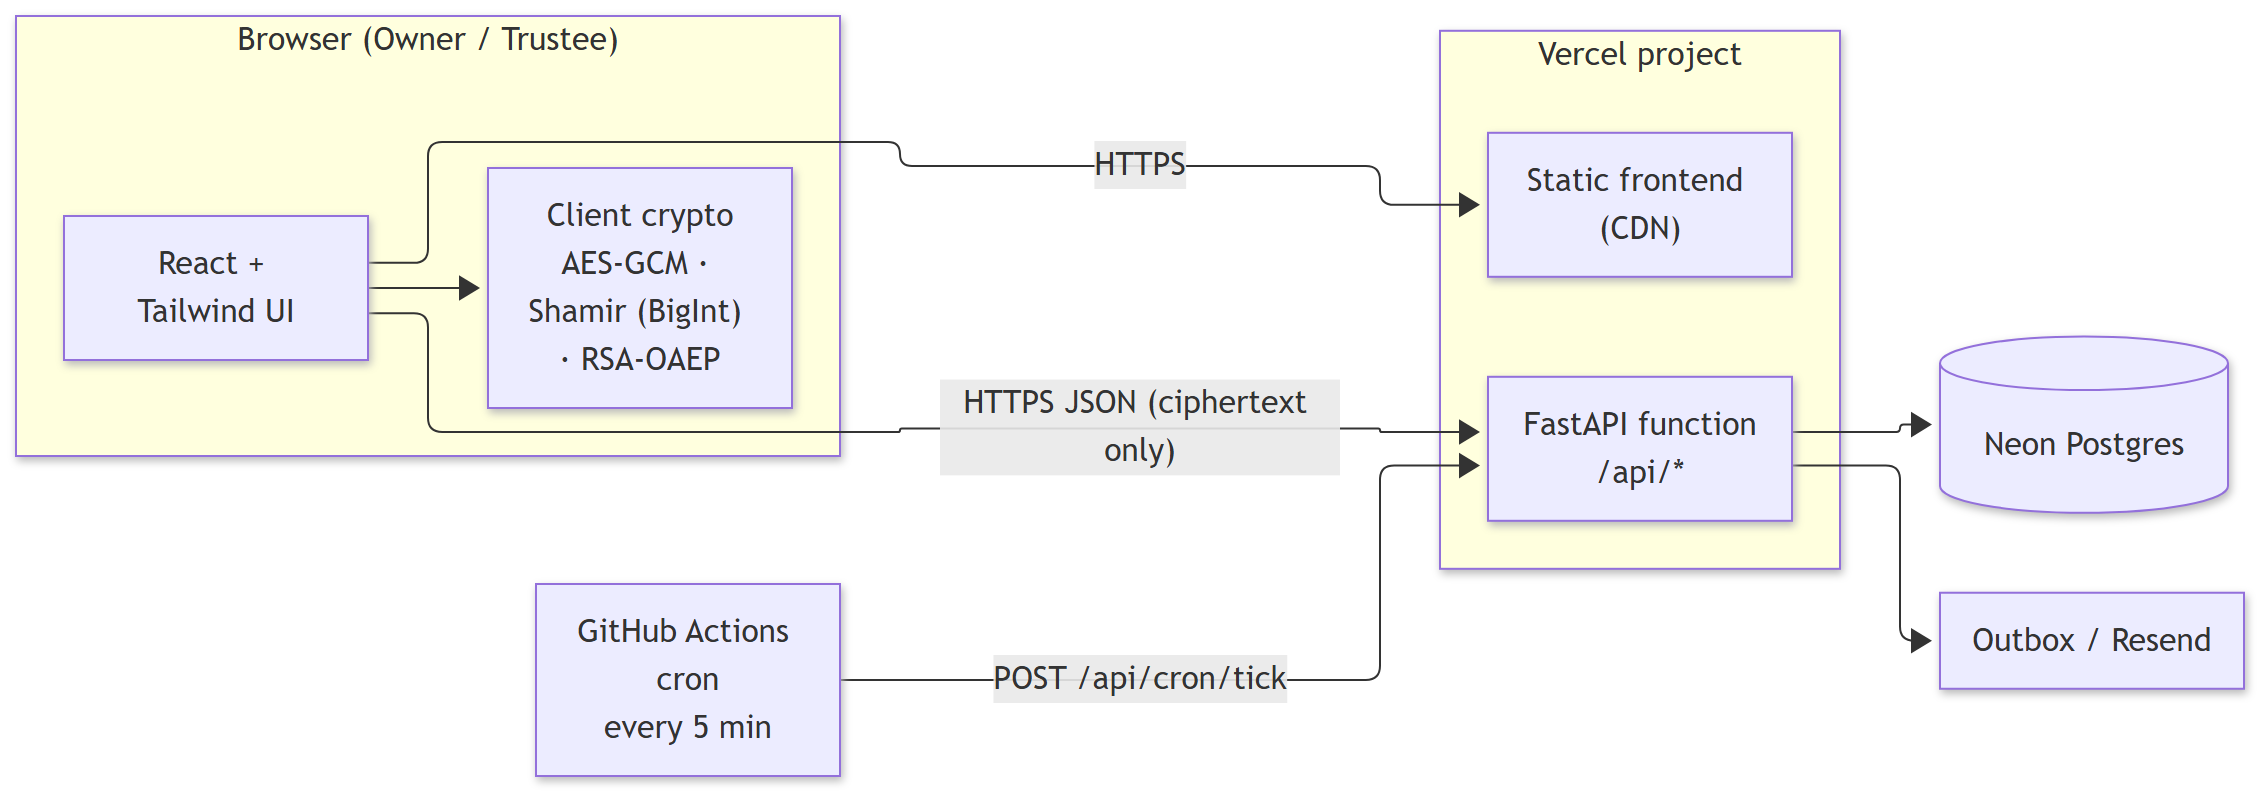
\includegraphics[width=\textwidth]{diagrams/architecture-2.png}
  \caption{Deployment architecture}
  \label{fig:architecture}
\end{figure}

\begin{figure}[htbp]
  \centering
  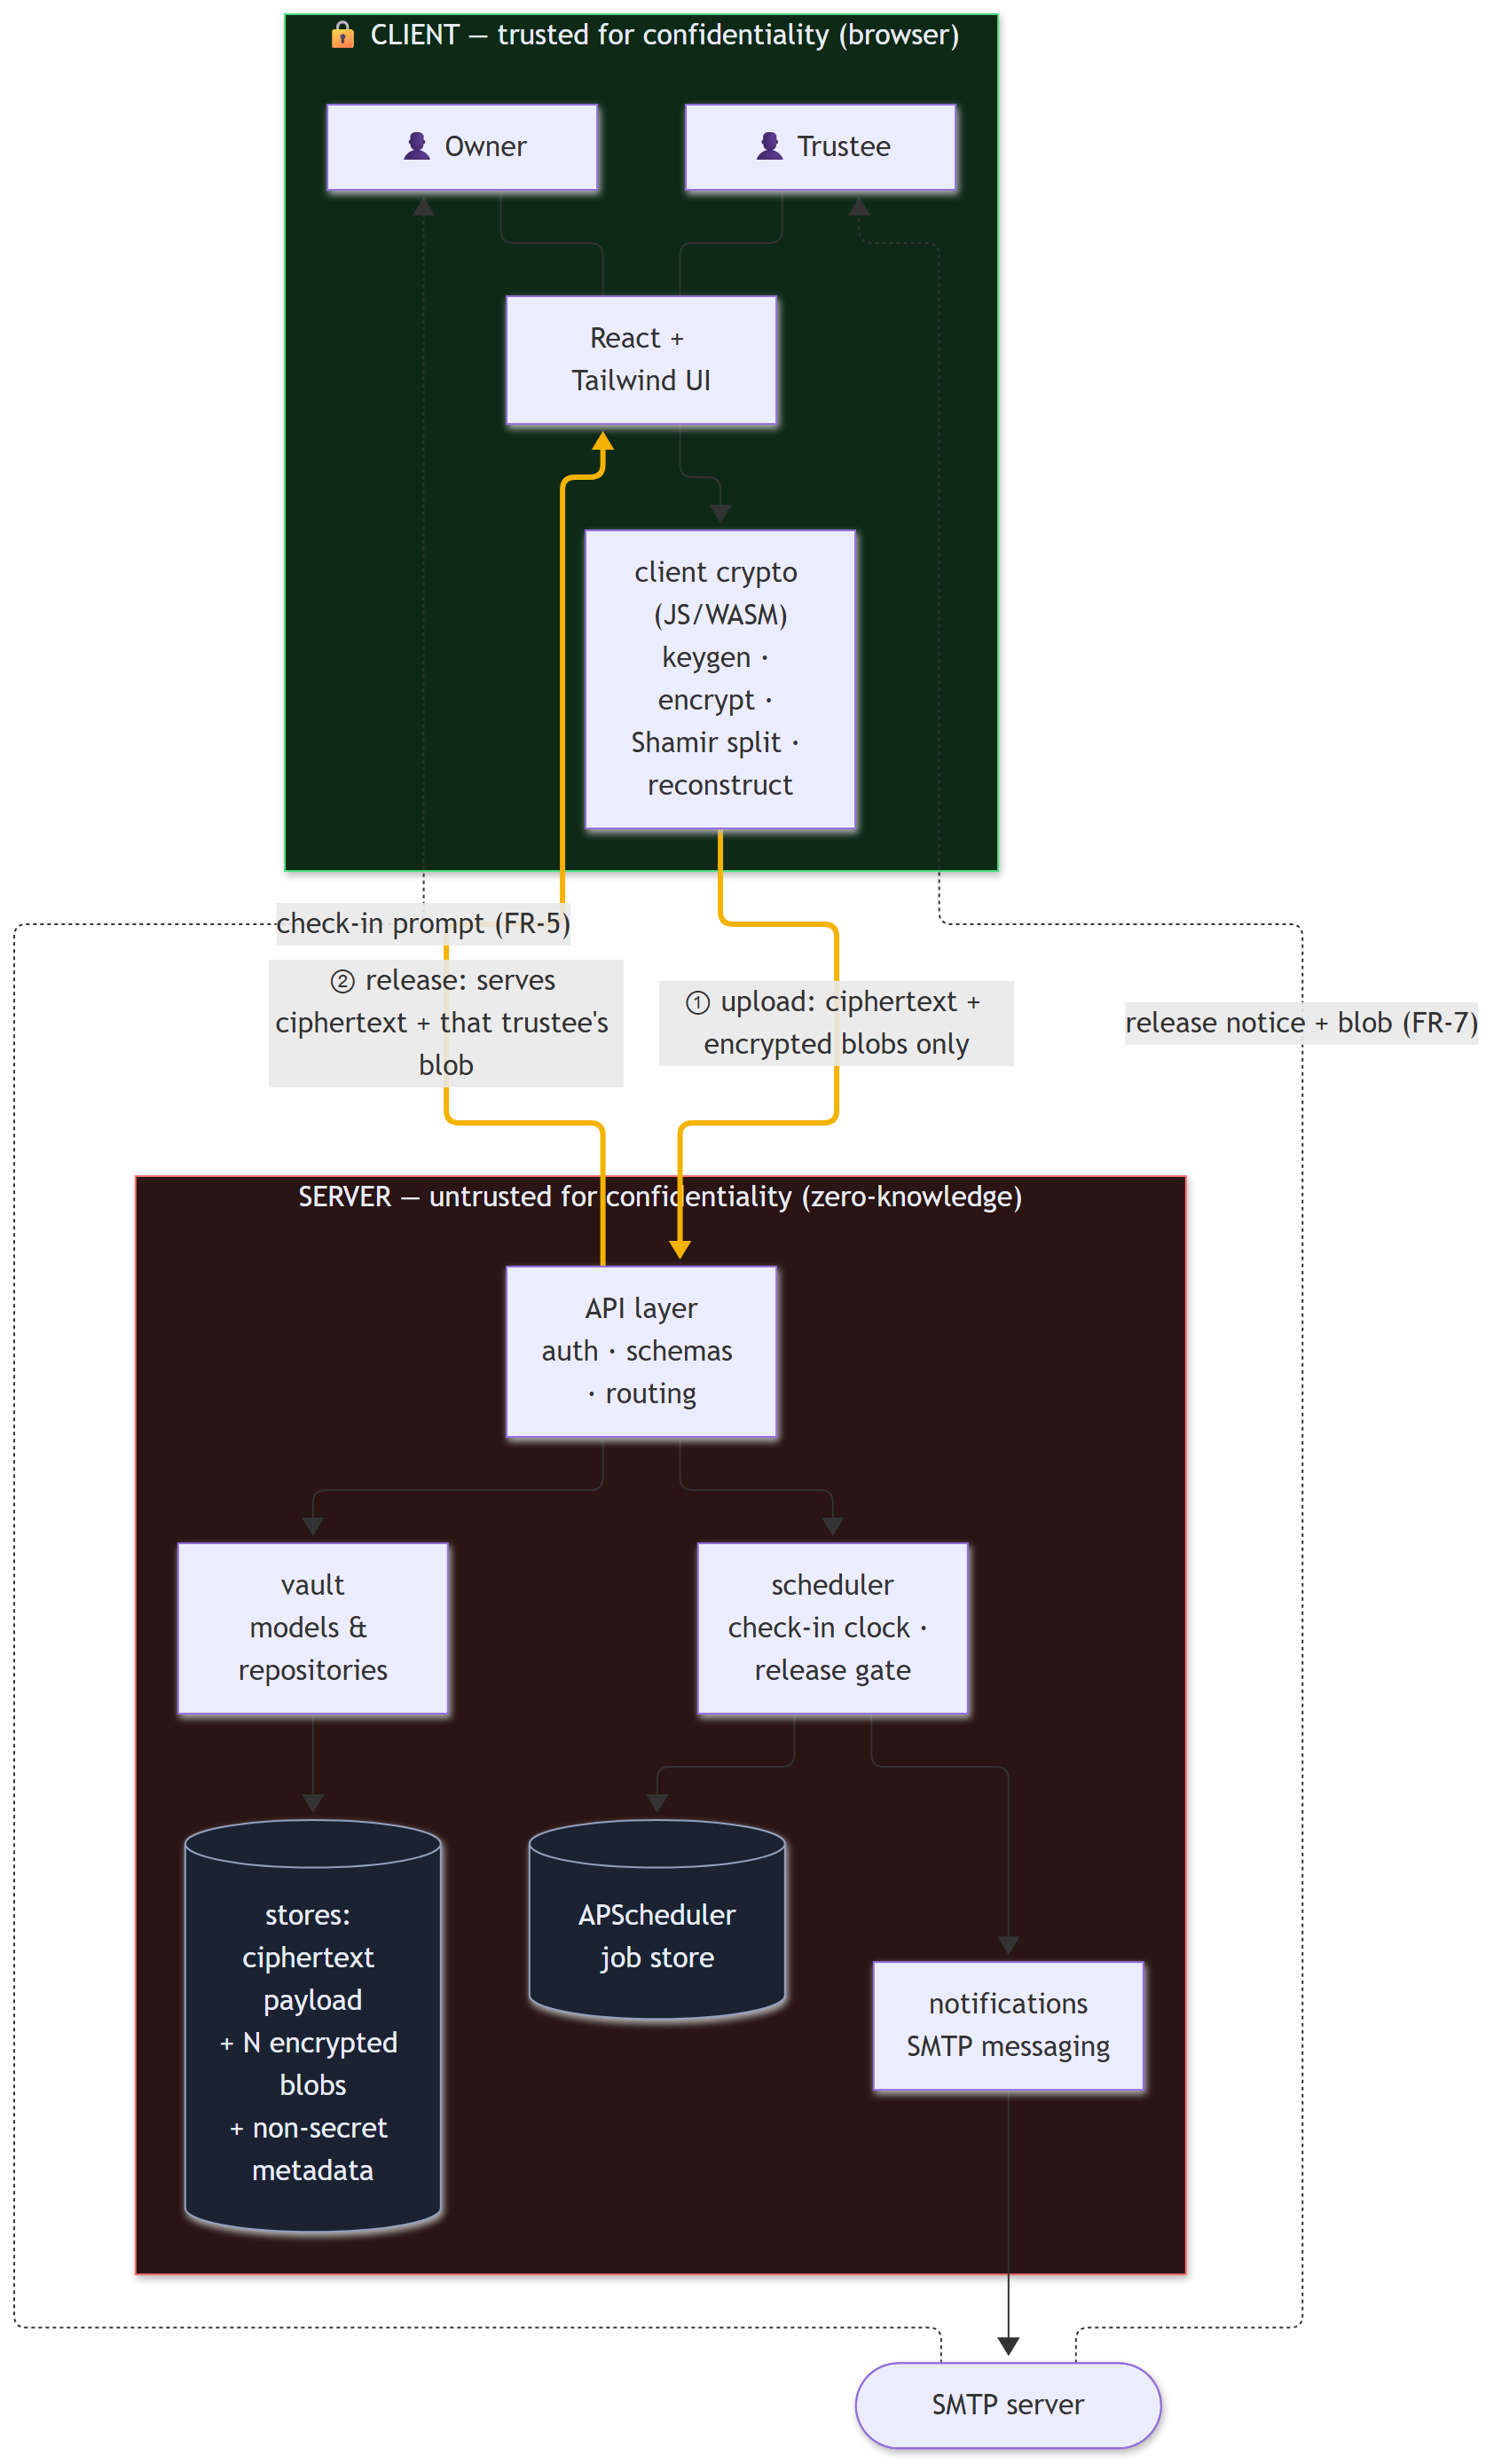
\includegraphics[height=0.72\textheight,width=\textwidth,keepaspectratio]{diagrams/architecture-1.png}
  \caption{Client/server trust boundary: only ciphertext and encrypted blobs cross it}
  \label{fig:trust-boundary}
\end{figure}

\subsection{High-Level Design}\label{sec:design-hld}

\paragraph{Components.} The browser hosts the user interface and the client
crypto module (AES-256-GCM, a hand-written Shamir implementation over
\code{BigInt}, and RSA-OAEP). The FastAPI application exposes authentication,
vault, check-in, trustee, cron and demo endpoints under
\code{/api}~\cite{fastapidocs}. Four domain packages sit behind it:
\code{crypto} (the authoritative specification and test oracle),
\code{scheduler} (the lifecycle), \code{vault} (SQLAlchemy models and
repositories~\cite{sqlalchemydocs}) and \code{notifications} (a transactional
outbox).

\paragraph{Trust model.} The server is trusted for scheduling and delivery,
never for confidentiality. The browser generates a random 256-bit key, encrypts
the payload, splits the key into $N$ shares and encrypts each share to its
trustee's RSA public key; the server receives only the results. Trustees
generate their keypairs in their own browsers and keep the private key as a
downloaded file. A server breach alone therefore reveals nothing; a breach of
confidentiality requires the server \emph{and} at least $K$ trustees. The
documented residual risks (for example, a malicious operator serving altered
client code) are discussed in Section~\ref{sec:results-analysis}.

\paragraph{Vault state machine.} Each vault moves through Setup, Active,
Warning, Grace and Released (Figure~\ref{fig:state-machine}). The decision is
made by a single pure function, \code{evaluate(clock, now)}, which releases a
vault only when the current time has reached the deadline plus the full grace
period with no confirmed check-in. A check-in from Active, Warning or Grace
returns the vault to Active; Released is terminal.

% The exported diagram figures/diagrams/vault-lifecycle-1.png is too wide to
% stay legible at text width, so the same diagram is redrawn here in TikZ.
\begin{figure}[htbp]
  \centering
  \resizebox{\textwidth}{!}{%
  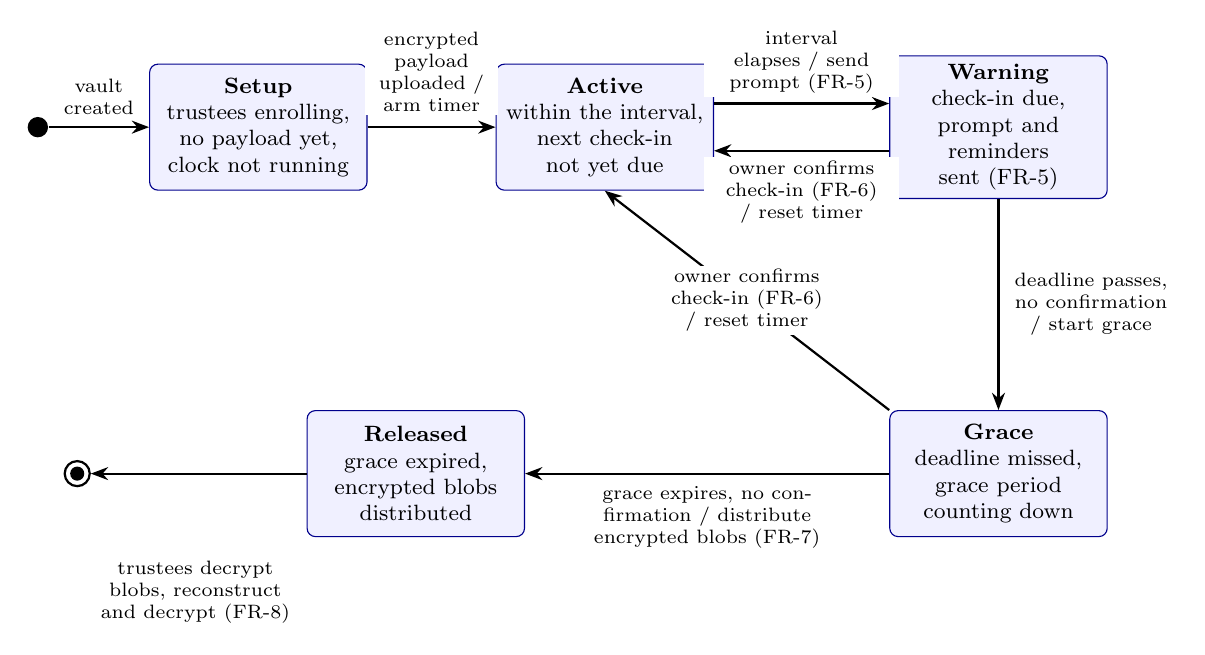
\begin{tikzpicture}[
      >={Stealth[length=2.2mm]}, font=\small,
      st/.style={draw=blue!55!black, rounded corners=3pt, fill=blue!6,
                 align=center, text width=2.55cm, minimum height=1.6cm,
                 inner sep=3pt, font=\footnotesize},
      lab/.style={font=\scriptsize, align=center, fill=white, inner sep=1.2pt},
      every edge/.style={draw, ->, thick}]
    \node[circle, fill, inner sep=2.6pt] (start) at (-0.9,0) {};
    \node[st] (setup)    at (1.9,0)   {\textbf{Setup}\\trustees enrolling, no payload yet, clock not running};
    \node[st] (active)   at (6.3,0)   {\textbf{Active}\\within the interval, next check-in not yet due};
    \node[st] (warning)  at (11.3,0)  {\textbf{Warning}\\check-in due, prompt and reminders sent (FR-5)};
    \node[st] (grace)    at (11.3,-4.4) {\textbf{Grace}\\deadline missed, grace period counting down};
    \node[st] (released) at (3.9,-4.4)  {\textbf{Released}\\grace expired, encrypted blobs distributed};
    \node[circle, draw, thick, inner sep=3.2pt] (end) at (-0.4,-4.4) {};
    \node[circle, fill, inner sep=1.8pt] at (end) {};

    \draw[->, thick] (start) -- node[lab, above=3pt, text width=1.2cm] {vault created} (setup);
    \draw[->, thick] (setup) -- node[lab, text width=1.6cm, above=4pt]
      {encrypted payload uploaded / arm timer} (active);
    \draw[->, thick] ([yshift=3mm]active.east) -- node[lab, text width=2.4cm, above=2pt]
      {interval elapses / send prompt (FR-5)} ([yshift=3mm]warning.west);
    \draw[->, thick] ([yshift=-3mm]warning.west) -- node[lab, text width=2.4cm, below=2pt]
      {owner confirms check-in (FR-6) / reset timer} ([yshift=-3mm]active.east);
    \draw[->, thick] (warning.south) -- node[lab, text width=2.1cm, right=2pt]
      {deadline passes, no confirmation / start grace} (grace.north);
    \draw[->, thick] (grace.north west) -- node[lab, text width=2.3cm, pos=0.5]
      {owner confirms check-in (FR-6) / reset timer} (active.south);
    \draw[->, thick] (grace.west) -- node[lab, text width=3.6cm, below=3pt]
      {grace expires, no confirmation / distribute encrypted blobs (FR-7)} (released.east);
    \draw[->, thick] (released.west) -- (end);
    \node[lab, text width=3.2cm, anchor=north] at ([xshift=-2.8cm,yshift=-0.25cm]released.south)
      {trustees decrypt blobs, reconstruct and decrypt (FR-8)};
  \end{tikzpicture}}
  \caption{Vault lifecycle state machine with its triggers and actions}
  \label{fig:state-machine}
\end{figure}

Figures~\ref{fig:seq-create} and~\ref{fig:seq-release} show the two principal
flows: creating and sealing a vault, and releasing and recovering it.
Figure~\ref{fig:data-model} shows the data model; the use-case view is
Figure~\ref{fig:use-case}.

\begin{sidewaysfigure}
  \centering
  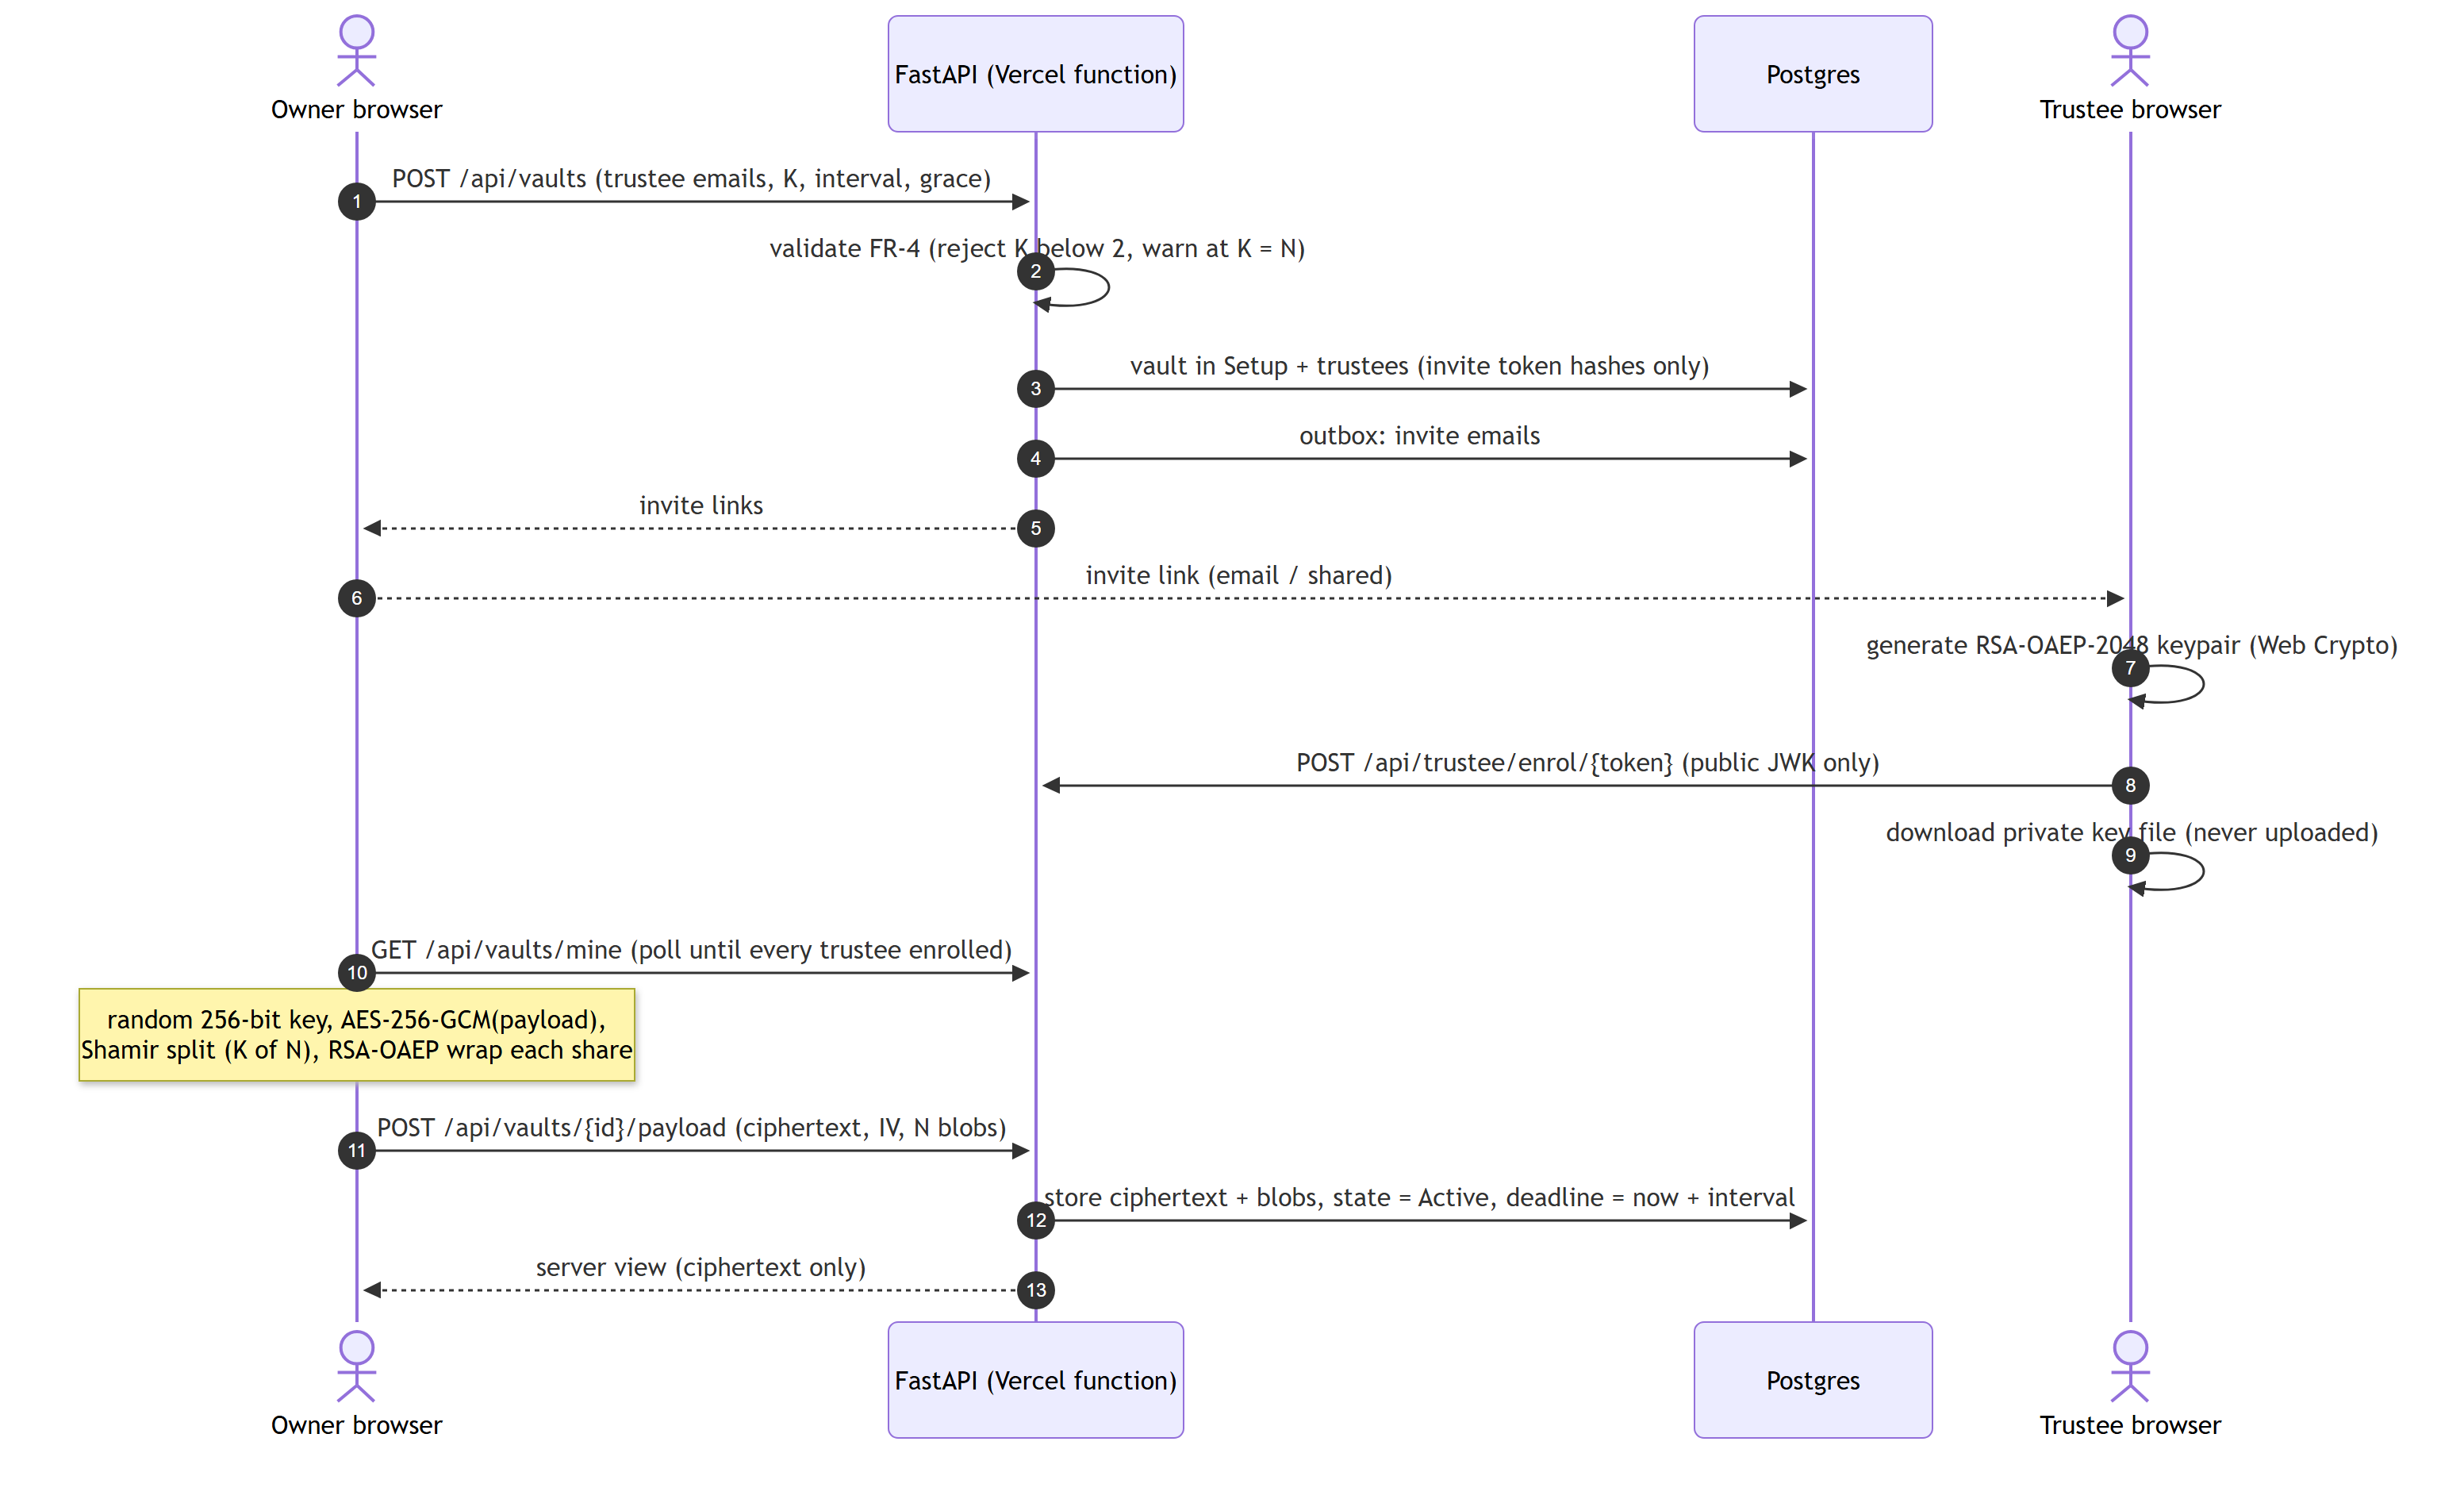
\includegraphics[width=\textheight,height=0.85\textwidth,keepaspectratio]{diagrams/sequences-1.png}
  \caption{Sequence: creating and sealing a vault}
  \label{fig:seq-create}
\end{sidewaysfigure}

\begin{sidewaysfigure}
  \centering
  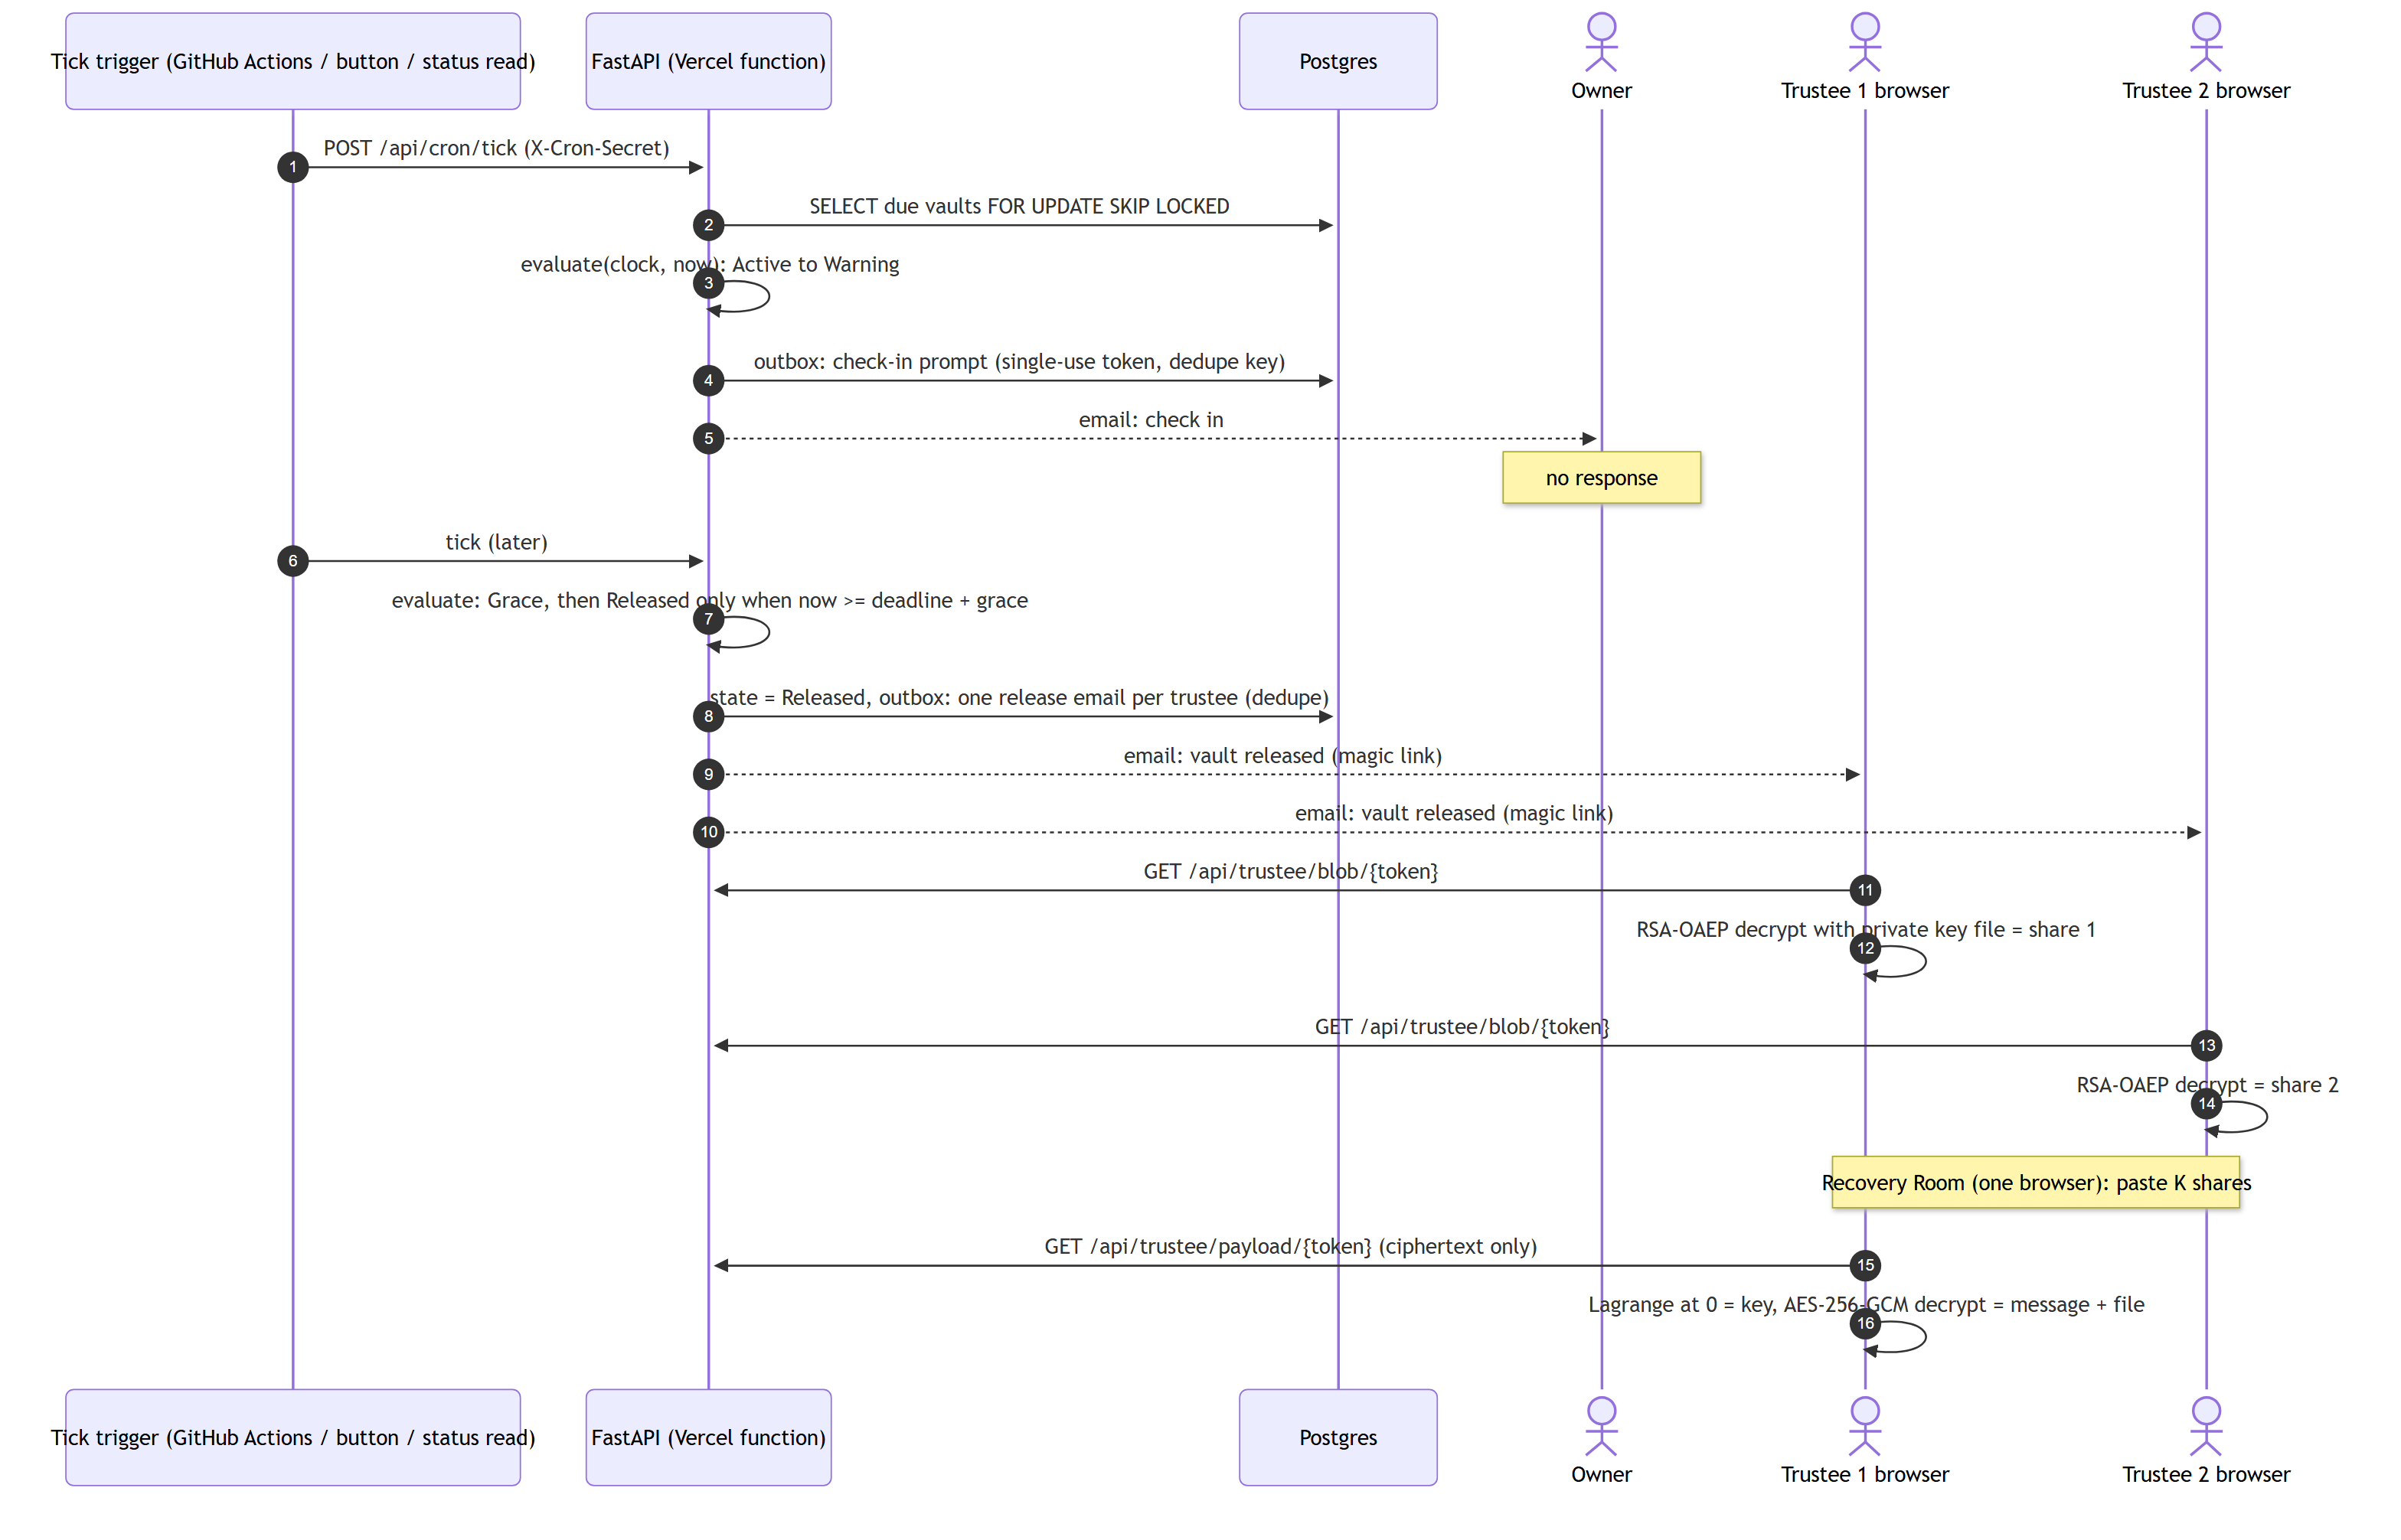
\includegraphics[width=\textheight,height=0.85\textwidth,keepaspectratio]{diagrams/sequences-2.png}
  \caption{Sequence: release and $K$-of-$N$ recovery}
  \label{fig:seq-release}
\end{sidewaysfigure}

\begin{figure}[htbp]
  \centering
  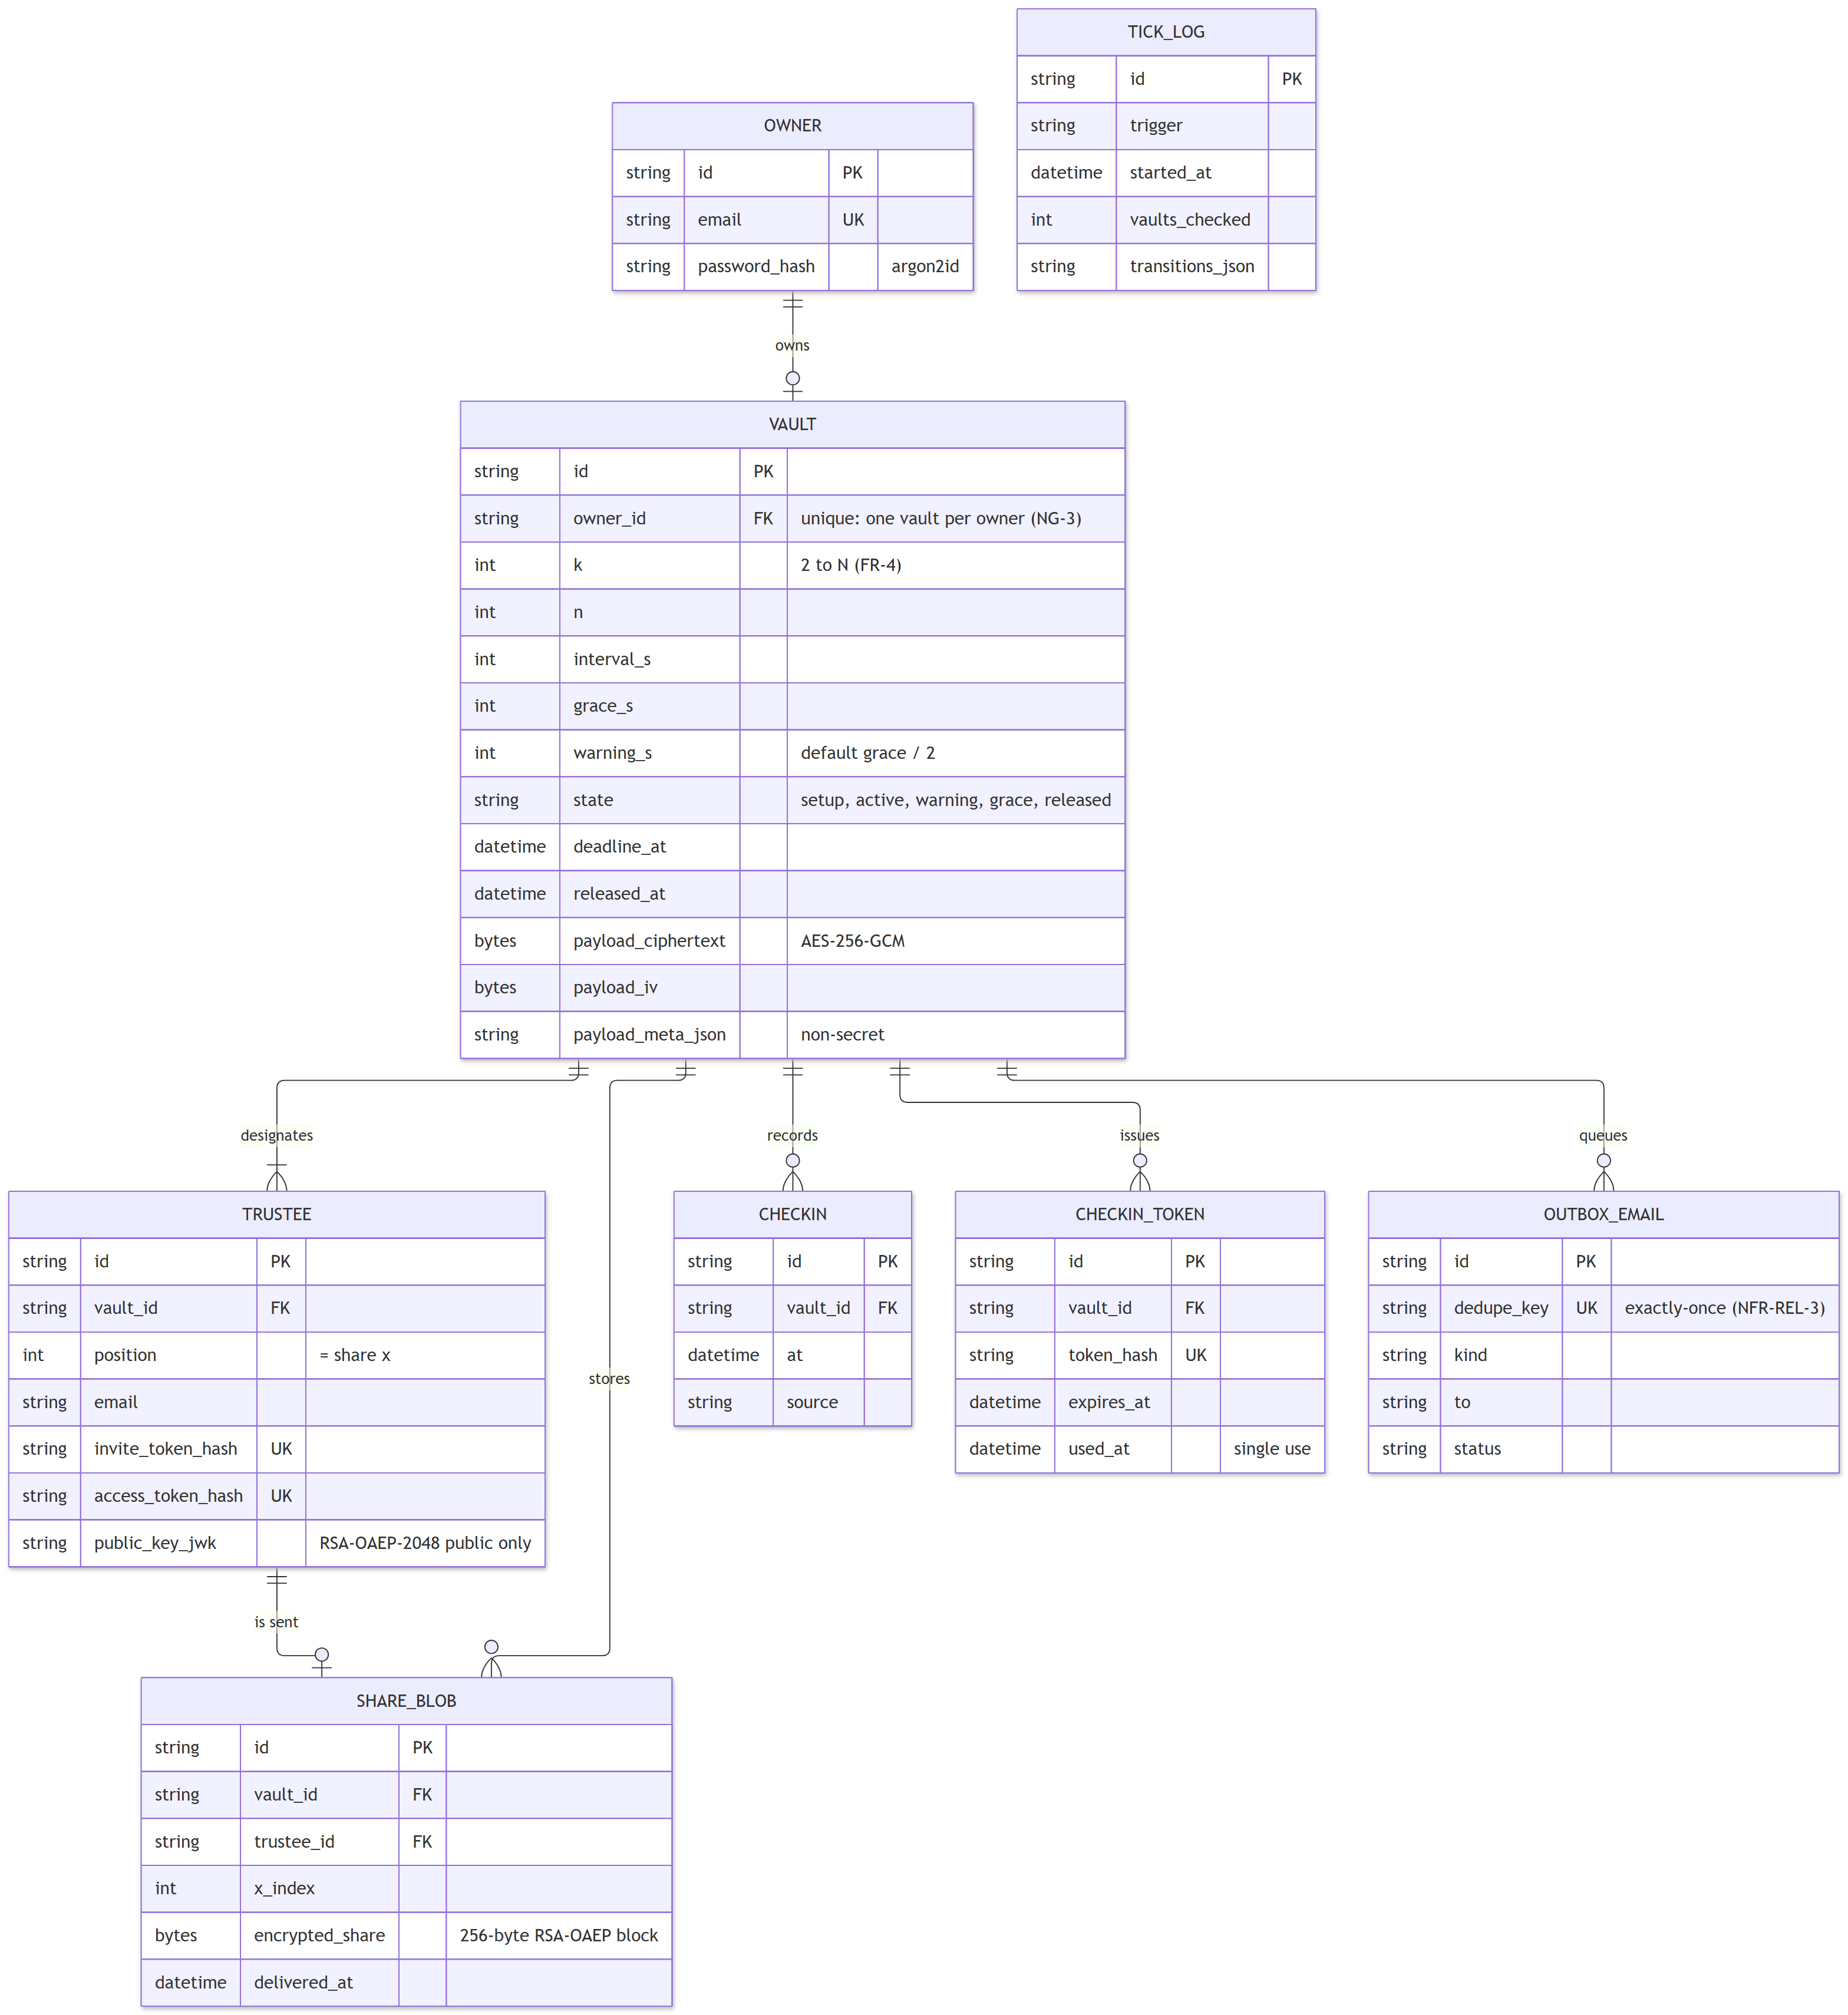
\includegraphics[width=\textwidth,height=0.75\textheight,keepaspectratio]{diagrams/data-model-1.png}
  \caption{Data model (SQLAlchemy entities)}
  \label{fig:data-model}
\end{figure}

\begin{figure}[htbp]
  \centering
  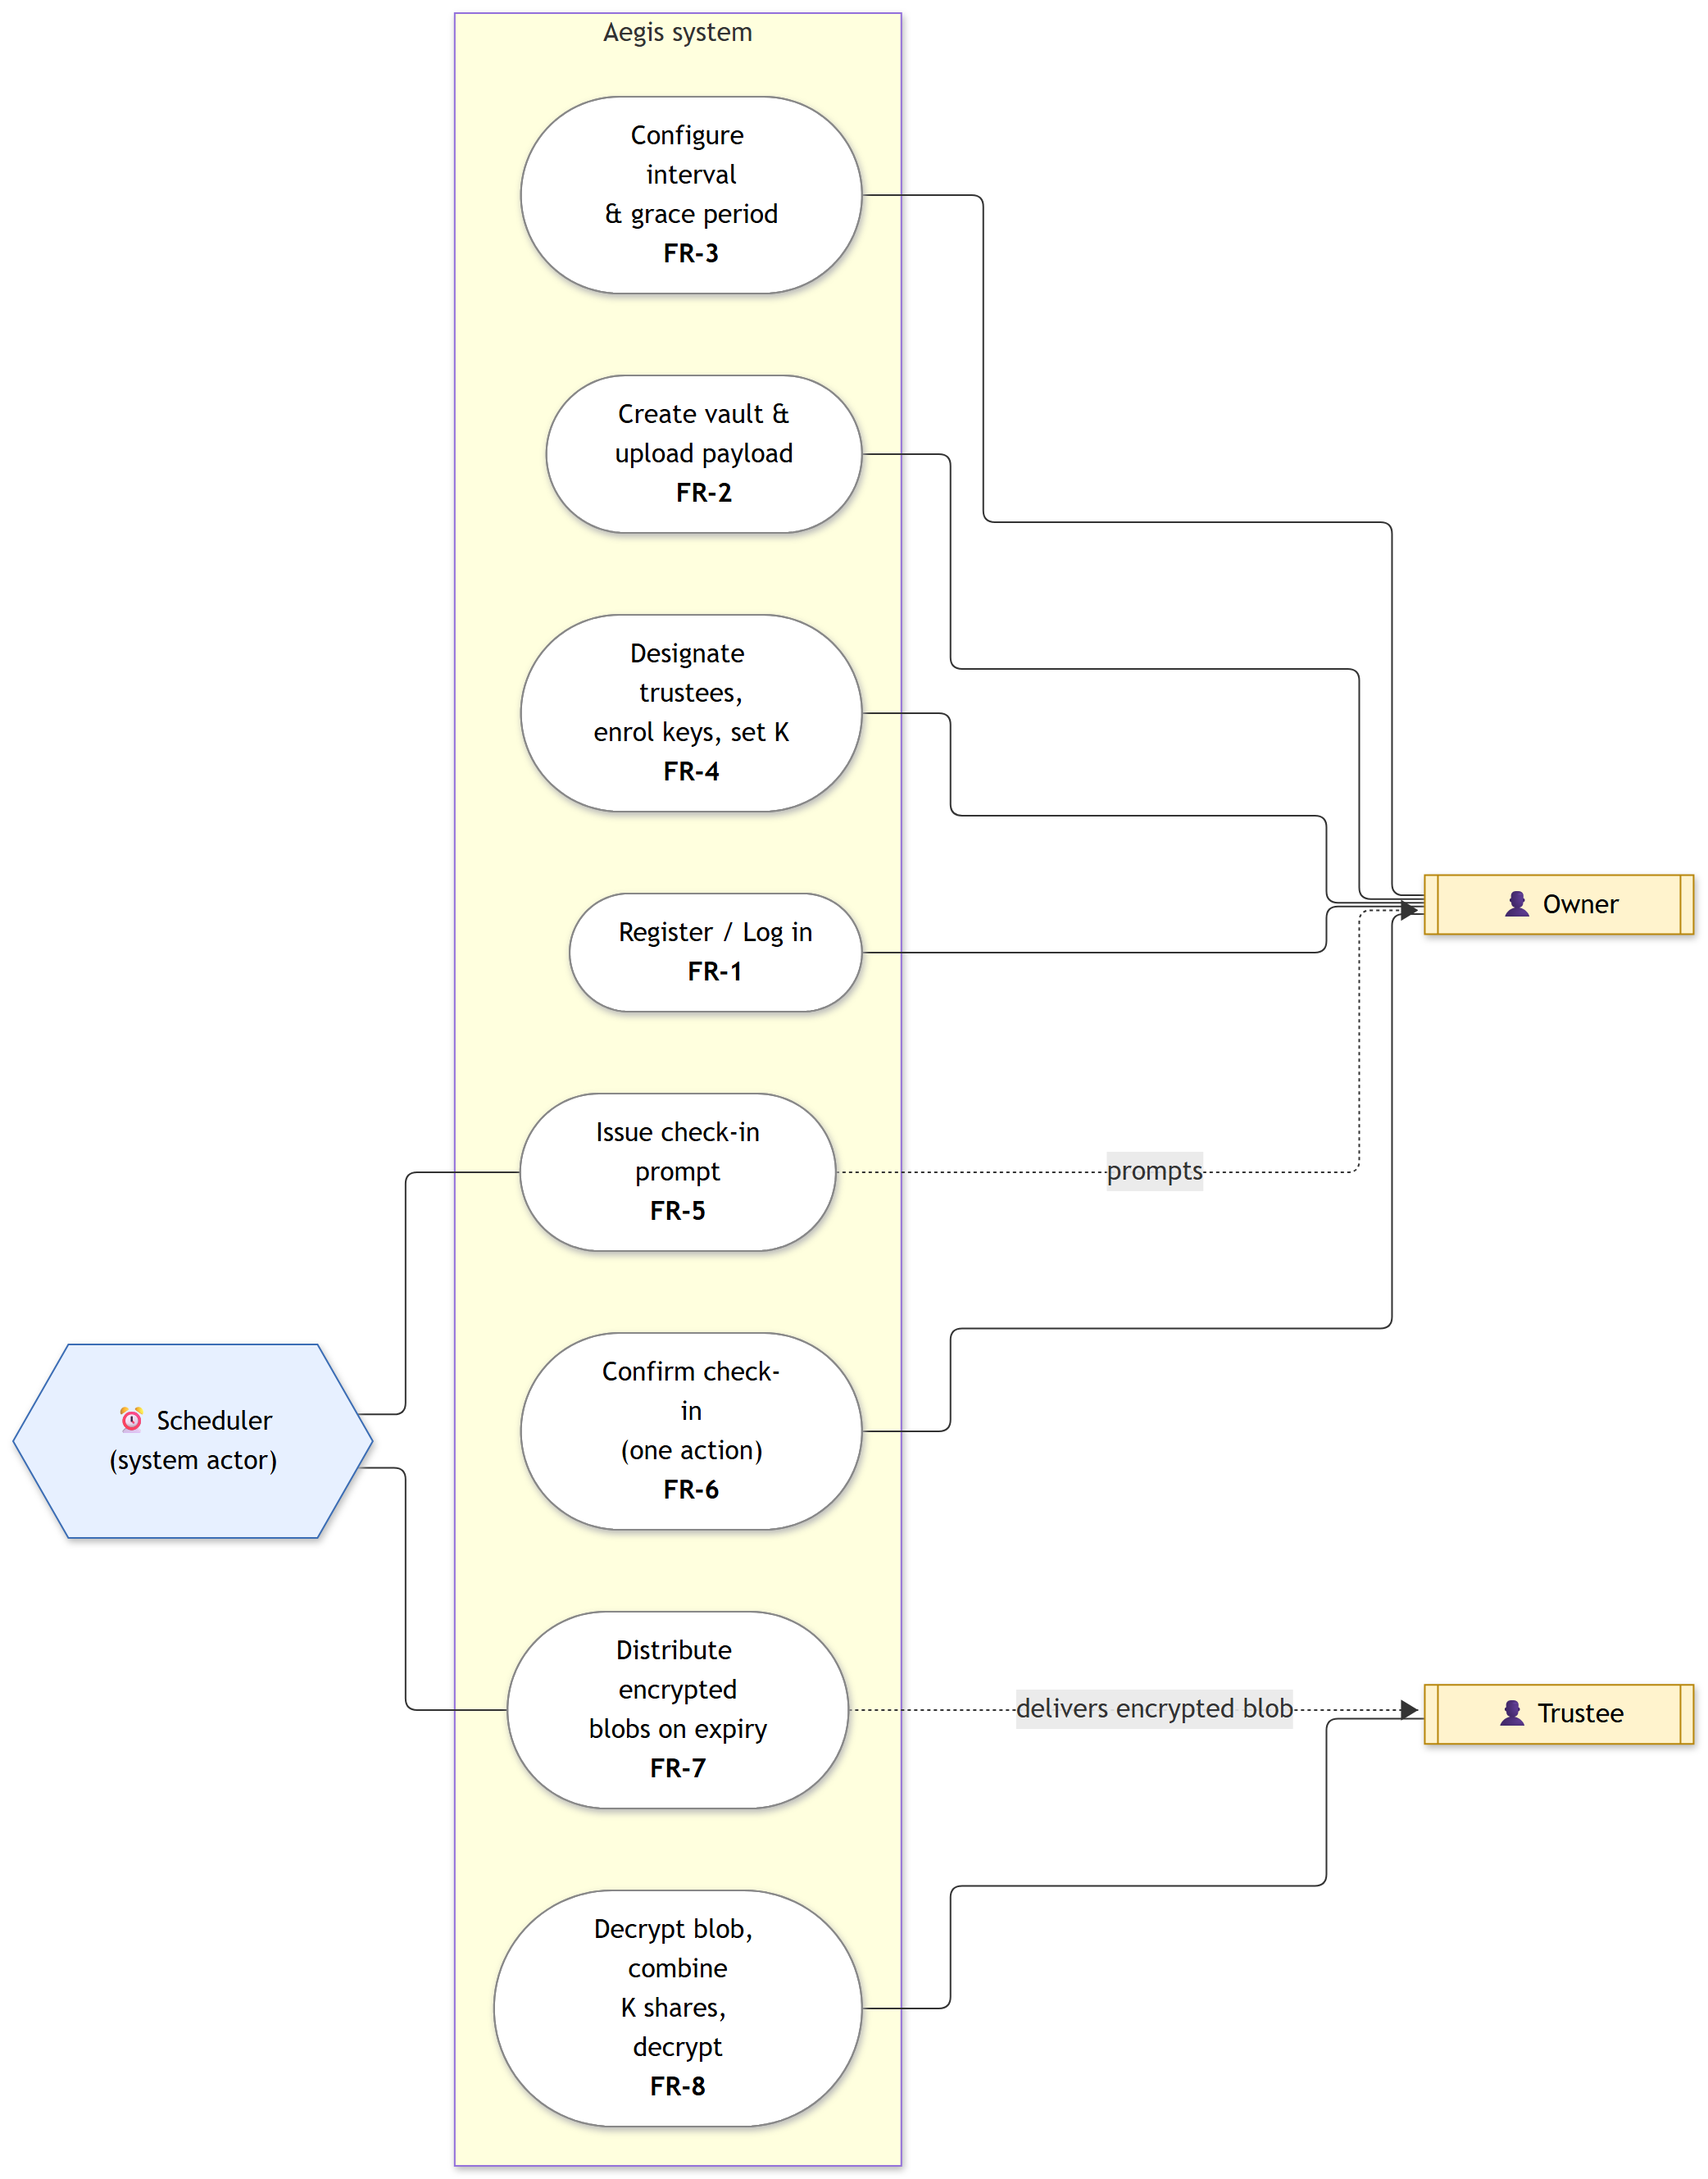
\includegraphics[height=0.68\textheight,width=\textwidth,keepaspectratio]{diagrams/use-case-1.png}
  \caption{Use-case diagram: Owner, Trustee and the time-triggered Scheduler}
  \label{fig:use-case}
\end{figure}

\subsection{Technical Stack}\label{sec:design-stack}

\begin{itemize}
  \item \textbf{Framework/Language:} Python~3.12 with FastAPI for the API;
    TypeScript with React~18, Vite~8 and Tailwind CSS~4 for the
    client~\cite{reactdocs}.
  \item \textbf{Database:} SQLAlchemy~2 with SQLite for local development and
    tests, and Postgres on Neon in production (\req{NFR-PORT-1}). Payloads are
    stored as ciphertext in the database, capped at about 1\,MB.
  \item \textbf{Tools:} Git and GitHub with feature branches and pull
    requests; GitHub Actions for continuous integration and the 5-minute
    scheduler trigger; Vercel for hosting; Playwright for end-to-end
    testing~\cite{playwrightdocs}; Lighthouse for page quality; ruff, ESLint
    and Prettier for code quality.
  \item \textbf{Libraries:} the browser's Web Cryptography API for
    AES-256-GCM~\cite{nist80038d} and RSA-OAEP-2048 with
    SHA-256~\cite{rfc8017,w3cwebcrypto}; \code{argon2-cffi} for password
    hashing~\cite{rfc9106}; PyJWT for session tokens; pytest,
    Hypothesis~\cite{maciver2019hypothesis} and Vitest for testing;
    self-hosted Instrument Sans and JetBrains Mono variable fonts (Fontsource)
    for the interface.
\end{itemize}

Table~\ref{tab:stack} summarises each technology choice and the reason for it.

\begin{table}[htbp]
  \centering
  \small
  \caption{Technology choices and their reasons}
  \label{tab:stack}
  \begin{tabularx}{\textwidth}{|L{2.3cm}|Y|Y|}
    \hline
    \textbf{Layer} & \textbf{Technology} & \textbf{Reason} \\ \hline
    Frontend       & React 18 + TypeScript + Vite 8 + Tailwind CSS 4 & Planned stack; static build served from Vercel's CDN \\ \hline
    Client crypto  & Web Crypto (AES-256-GCM, RSA-OAEP-2048/SHA-256) & Built into browsers; no third-party crypto library on the client \\ \hline
    Secret sharing & Hand-written Shamir over $\mathrm{GF}(2^{521}-1)$ & SRS constraint; Python and TypeScript versions bound by shared test vectors \\ \hline
    Backend        & Python 3.12 + FastAPI as a Vercel Python function & Planned stack; same origin as the frontend \\ \hline
    Database       & SQLAlchemy 2; SQLite locally, Neon Postgres in production & \req{NFR-PORT-1}; serverless functions have no persistent disk \\ \hline
    Scheduler      & Pure \code{evaluate()} + idempotent \code{POST /api/cron/tick} & Serverless functions keep no process alive, so no APScheduler \\ \hline
    Tick triggers  & GitHub Actions (5 min), Demo Console button, lazy due-checks, daily Vercel Cron & Hobby-plan Vercel Cron runs at most once a day \\ \hline
    Email          & Outbox + \code{EmailSender} (log / Resend) & Demo works without a verified email domain \\ \hline
    Auth           & argon2id + JWT in an httpOnly, SameSite=Lax cookie & \req{NFR-SEC-3} \\ \hline
    Testing        & pytest, Hypothesis, pytest-cov, Vitest, Playwright, Lighthouse & \req{NFR-MAINT-1} and the demo script as a test \\ \hline
  \end{tabularx}
\end{table}

\section{Implementation Details}\label{sec:design-implementation}

\subsection[Module 1: Core Functionality]{Module 1: Core Functionality ---
Client-Side Encryption and Shamir's Secret Sharing}\label{sec:design-module1}

\paragraph{Finite field.} All arithmetic is carried out modulo the Mersenne
prime $p = 2^{521}-1$, which is large enough to hold a 256-bit AES key as a
single field element. Division is multiplication by a modular inverse
(Fermat's little theorem in TypeScript, Python's three-argument \code{pow} in
the oracle).

\paragraph{Polynomial construction.} To split a key $S$ with threshold $K$,
the client draws $K-1$ coefficients uniformly at random from the field and
forms
\[
  f(x) = S + a_1 x + a_2 x^2 + \dots + a_{K-1} x^{K-1} \pmod p,
\]
so that $f(0) = S$. Trustee $i$ receives the point $\bigl(i, f(i)\bigr)$ for
$i = 1,\dots,N$; $x = 0$ is never used because $f(0)$ is the secret.

\paragraph{Reconstruction.} Any $K$ points determine a unique polynomial of
degree at most $K-1$, so the secret is recovered by Lagrange interpolation
evaluated at zero:
\begin{equation}
  S \;=\; \sum_{i} y_i \prod_{j \neq i} \frac{x_j}{x_j - x_i} \pmod p .
  \label{eq:lagrange}
\end{equation}
With only $K-1$ points, every candidate secret is consistent with exactly one
polynomial through those points, so the shares reveal nothing about
$S$~\cite{shamir1979}. A Hypothesis property test checks this directly: for
random $K-1$ shares and a random candidate secret, it constructs coefficients
that the real split code turns into exactly those shares.

\paragraph{Share encoding and wrapping.} A share is encoded as 68 bytes (a
version byte, the $x$-coordinate and a 66-byte $y$) and encrypted to its
trustee's RSA-OAEP-2048 public key, producing a 256-byte blob; this fits
RSA-OAEP-SHA-256's 190-byte plaintext limit. Shares that trustees exchange in
the Recovery Room use the text form
\code{aegis-share:v1:<x>:<y-base64url>}. The payload is encrypted with
AES-256-GCM using the vault identifier as associated data, so a ciphertext
cannot be opened as another vault's.

\paragraph{Two implementations, one specification.} The Python package
\code{code/crypto} is the authoritative specification and test oracle; it
emits a versioned file of known-answer vectors (Shamir splits from known
coefficients, reconstructions, AES-GCM and RSA-OAEP cases). The TypeScript
client must reproduce every vector, and continuous integration fails if the two
disagree. Result: 13/13 matched.

Algorithms~\ref{alg:seal} and~\ref{alg:recover} give the client-side sealing
and recovery steps.

\begin{algorithm}[H]
  \caption{\textsc{Seal}: client-side sealing of a vault}
  \label{alg:seal}
  \begin{algorithmic}[1]
    \Function{Seal}{$\mathit{payload}, \mathit{trustees}, K$}
      \State $\mathit{key} \gets$ 32 random bytes;\; $\mathit{iv} \gets$ 12 random bytes
      \State $\mathit{aad} \gets \text{`aegis-vault:v1:'} \parallel \mathit{vault\_id}$
      \State $\mathit{ct} \gets \textsc{AES-256-GCM-Encrypt}(\mathit{key}, \mathit{iv}, \mathit{payload}, \mathit{aad})$
      \State $a_1,\dots,a_{K-1} \gets$ uniform random field elements
      \For{$i \gets 1$ \textbf{to} $N$}
        \State $\mathit{share}_i \gets \bigl(i, f(i)\bigr)$ where $f(x) = \mathrm{int}(\mathit{key}) + a_1x + \dots + a_{K-1}x^{K-1} \bmod p$
        \State $\mathit{blob}_i \gets \textsc{RSA-OAEP-Encrypt}(\mathit{trustee}_i.\mathit{public\_key},\ \textsc{Encode}(\mathit{share}_i))$
      \EndFor
      \State \textsc{Upload}$(\mathit{ct}, \mathit{iv}, \mathit{blob}_1,\dots,\mathit{blob}_N)$;\; \textsc{Wipe}$(\mathit{key})$
    \EndFunction
  \end{algorithmic}
\end{algorithm}

\begin{algorithm}[H]
  \caption{\textsc{Recover}: $K$-of-$N$ recovery in the Recovery Room}
  \label{alg:recover}
  \begin{algorithmic}[1]
    \Function{Recover}{$\mathit{shares}, K, \mathit{ct}, \mathit{iv}$}
      \If{$|\mathit{shares}| < K$}
        \State \Return report `not enough shares'
      \EndIf
      \State $S \gets \sum_i y_i \prod_{j \neq i} x_j / (x_j - x_i) \bmod p$
      \State $\mathit{key} \gets$ 32-byte big-endian encoding of $S$
      \Statex \hspace{\algorithmicindent}\hspace{\algorithmicindent}\textit{(fails if $S$ does not fit: wrong or too few shares)}
      \State \Return $\textsc{AES-256-GCM-Decrypt}(\mathit{key}, \mathit{iv}, \mathit{ct}, \mathit{aad})$
      \Statex \hspace{\algorithmicindent}\hspace{\algorithmicindent}\textit{(GCM authentication fails on any error)}
    \EndFunction
  \end{algorithmic}
\end{algorithm}

\paragraph{Worked example (toy prime $p = 31$).} Take secret $S = 13$,
threshold $K = 3$ and $N = 5$, with random coefficients $a_1 = 7$ and
$a_2 = 4$, so
\[
  f(x) = 13 + 7x + 4x^2 \pmod{31}.
\]
The five shares are $(1, 24)$, $(2, 12)$, $(3, 8)$, $(4, 12)$, $(5, 24)$.
Using the shares at $x = 1, 3, 5$, the Lagrange basis values at zero are
$\ell_1(0) = 29$, $\ell_2(0) = 22$, $\ell_3(0) = 12 \pmod{31}$, and
\[
  \sum_i y_i\,\ell_i(0) = 24\cdot 29 + 8\cdot 22 + 24\cdot 12 \equiv 13 \pmod{31},
\]
which is the secret.

With only two shares, $(1, 24)$ and $(3, 8)$, every candidate secret fits some
quadratic: for example $S = 0$ gives $f(x) = 0 + 14x + 10x^2$; $S = 5$ gives
$f(x) = 5 + 28x + 22x^2$; $S = 22$ gives $f(x) = 22 + 26x + 7x^2$ (all
mod~$31$), each passing through both known shares. Two shares therefore say
nothing about $S$.

\subsection{Module 2: Secondary Features}\label{sec:design-module2}

\paragraph{Scheduler and tick design.} The lifecycle is decided by the pure
function \code{evaluate(clock, now)}, which returns the new state and the
actions owed on the way (check-in prompt, grace reminder, release). It moves
only forward, so a backward clock jump never undoes a transition, and it
catches up through missed transitions in order after an outage. The SRS fixes
only the interval and grace period (\req{FR-3}); the implementation places the
Warning-to-Grace boundary inside the grace window (by default at its
midpoint), so the release instant remains exactly the deadline plus the grace
period. A late check-in, arriving at or after that instant, is refused, so the
outcome never depends on whether a tick happened to run first.

\paragraph{Transactional tick and exactly-once release.} \code{tick()} loads
due vaults with \code{SELECT ... FOR UPDATE SKIP LOCKED} on Postgres (SQLite
takes the write lock up front), applies \code{evaluate} to the locked rows and
writes the state change and the outbox rows in one transaction. Each outbox
row has a unique deduplication key, for example
\code{release:<vault>:<trustee>}, so a release is recorded exactly once even
when two ticks race (\req{NFR-REL-3}). Deadlines live in the database, so a
restarted process resumes where the previous one stopped (\req{NFR-REL-2}).
Ticks come from GitHub Actions every five minutes, a Demo Console button, a
cheap due-check whenever an owner or trustee status endpoint is read, and a
daily Vercel Cron backstop.

\paragraph{Check-in tokens.} Prompt emails carry a one-click link with a
single-use, expiring token; only its SHA-256 hash is stored. The link's
\code{GET} request only previews the token; the page confirms with a
\code{POST}, so email security scanners that pre-fetch links cannot check in on
the owner's behalf (threat \req{T-5}).

\paragraph{Trustee enrolment.} Each trustee opens an invitation link; their
browser generates an RSA-OAEP-2048 keypair, uploads only the public key and
forces a download of the private-key file (optionally also kept in IndexedDB).
The API rejects any key containing private-key fields. \req{FR-4} is enforced
on the server and in the user interface: $K$ below 2 is rejected, $K = N$
produces a warning that losing any trustee makes the vault unrecoverable, and
the loss tolerance $N - K$ is displayed.

\paragraph{Notification service.} Email is a strategy behind an
\code{EmailSender} interface: \code{log} mode records every message in an
in-app Outbox (used in the demonstration), and \code{resend} mode also sends
through Resend.

\paragraph{Frontend pages.} A landing page; registration and login; an owner
dashboard with a live countdown on the server's clock and a single
\enquote{I'm OK --- check in} button; a vault wizard that asks for the secret
only after every trustee has enrolled and then shows exactly what the server
received; the one-click check-in page; trustee enrolment and portal pages; a
Recovery Room that reconstructs and decrypts entirely in the browser; and a
token-protected Demo Console with the Outbox, tick log, server view and
measured results.

\paragraph{Deployment.} One Vercel project builds the Vite frontend as static
files and runs \code{api/index.py} as a Python function; rewrites send
\code{/api/*} to the function and all other paths to the single-page app.

\section{Work Completed for the Final Product}\label{sec:design-final}

\subsection{Production Deployment and Demonstration Tooling}

The application runs in production on Vercel with a Neon Postgres database.
Secrets (the session signing key, the cron token and the Demo Console token)
are set as Vercel environment variables for the production and preview
environments, and \code{GET /api/health} reports the database in use and the
deployed Git commit, which was used to confirm each release. The GitHub
Actions workflow calls the tick endpoint every five minutes with the cron
token.

Because a demonstration vault is eventually released by design, the script
\code{scripts/seed\_demo.py} prepares a fresh demonstration against any
deployment through the public API only: it registers the owner, creates three
trustees, generates each trustee's RSA keypair locally (the server again
receives only public keys), seals a 2-of-3 vault with a chosen interval and
grace period, and writes each trustee's private-key file and portal link to a
local folder. Together with the Demo Console's \enquote{Reset demo data} action
this gives a repeatable demonstration with a known starting state.

\subsection{User Interface Redesign}

The interface was redesigned for the final evaluation around a small design
system rather than per-page styling:

\begin{itemize}
  \item \textbf{Design tokens.} Colours for the page, translucent surfaces,
    borders, shadows and background glows are CSS custom properties defined
    once for the light theme and once for the dark theme, so every component
    follows the active theme without per-component dark-mode rules.
  \item \textbf{Glass surfaces.} Three surface utilities (\code{glass},
    \code{glass-strong} and \code{glass-inset}) combine a translucent fill,
    a background blur, a hairline border and a soft shadow. Browsers without
    \code{backdrop-filter}, and users who ask their system for reduced
    transparency, get opaque surfaces instead, so text contrast never depends
    on what is behind a panel.
  \item \textbf{Shared components.} Buttons, cards, page headers, alerts,
    form fields, state badges and the countdown are implemented once in a
    shared module and used by every page. Lifecycle states keep one colour
    scheme everywhere (Active green, Warning amber, Grace orange, Released
    red), and the Warning and Grace badges pulse to draw attention.
  \item \textbf{Typography.} Instrument Sans for text and JetBrains Mono for
    labels, timers and identifiers, both self-hosted so no third-party font
    service sees the visitor.
  \item \textbf{Landing page.} The hero illustrates the lifecycle and a 2-of-3
    share split, and a results strip shows measured values (early releases,
    zero-knowledge findings, cross-language vectors and live check-in p95)
    read from the same metrics file that feeds this report, so the page cannot
    drift from the measurements.
  \item \textbf{Themes and small screens.} A header switch cycles Light, Dark
    and System; the choice is stored in the browser and applied by an inline
    script before the first paint, so pages never flash the wrong theme, and
    System follows the operating system's preference as it changes. On phones
    the navigation is a single swipeable row and the header scrolls away, so
    content starts near the top of the screen.
\end{itemize}

Every label, test identifier and button text used by the end-to-end test was
kept, so the automated demonstration script verified the redesign unchanged
(Section~\ref{sec:results-testing}).

\subsection{Quality Fixes and Dependency Maintenance}

\begin{itemize}
  \item \textbf{Search engines.} A real \code{robots.txt} is now served; the
    prototype answered that path with the single-page-app fallback, which cost
    the SEO score (Table~\ref{tab:results}).
  \item \textbf{Accessibility.} Re-running Lighthouse on the final build found
    one muted label on the landing page with a contrast ratio of 3.25:1 in the
    dark theme (4.5:1 required); its colour was corrected and the local
    re-run scored 100 for accessibility.
  \item \textbf{Dependencies.} \code{npm audit} advisories in development
    tools (ESLint, typescript-eslint and the diagram exporter's Mermaid) were
    cleared by upgrading to the lowest fixed versions. One moderate advisory
    remains in React Router~6, which is fixed only in the next major version;
    the upgrade is recorded as future work rather than risked just before the
    evaluation.
\end{itemize}

\subsection{Software Engineering Process}\label{sec:design-process}

The project followed the incremental 12-week plan in
\code{docs/plan/twelve-week-plan.md}: requirements and scaffolding (Week~1),
the zero-knowledge trust model and threat model (Week~2), the prototype
(Week~8) and the final product (Week~12)~\cite{pressman2020}. All work was
done on feature branches with small conventional commits and merged through
pull requests: the prototype (\#1), the live deployment results and report
(\#2), the user-interface redesign (\#3) and the dependency upgrades (\#4).
Continuous integration runs ruff, pytest with a coverage gate, ESLint, Vitest
(including the cross-language vectors), the production build and the
end-to-end test on every push, and each of the four pull requests was merged
with all of these checks passing. Vercel builds a preview deployment for every pull request and
deploys \code{main} to production. Requirements are traced to modules and
tests as shown in Table~\ref{tab:traceability}.

\begin{table}[htbp]
  \centering
  \footnotesize
  \caption{Requirement traceability: requirement $\rightarrow$ module $\rightarrow$ test}
  \label{tab:traceability}
  \begin{tabularx}{\textwidth}{|L{2.7cm}|Y|Y|}
    \hline
    \textbf{Requirement} & \textbf{Module} & \textbf{Verified by} \\ \hline
    FR-1, NFR-SEC-3 & \code{code/api/routes/auth.py}, \code{security.py} & \code{test\_api.py} (register/login, argon2id hash, cookie flags) \\ \hline
    FR-2, FR-2a, NFR-SEC-1, NFR-SEC-5 & \code{frontend/src/crypto/vault.ts} & \code{vault.test.ts}; \code{inspect\_server\_store.py} \\ \hline
    FR-3, FR-4 & \code{code/api/routes/vaults.py}; \code{VaultNew.tsx} & \code{test\_api.py} ($K<2$, $K=N$, interval); E2E step 3 \\ \hline
    FR-5, FR-7 & \code{code/scheduler/state.py}, \code{tick.py} & \code{test\_scheduler\_state.py}, \code{test\_scheduler\_tick.py} \\ \hline
    FR-6, NFR-USE-1 & \code{code/api/routes/checkin.py}; \code{CheckinLink.tsx} & \code{test\_api.py}; E2E (emailed link) \\ \hline
    FR-8, NFR-SEC-2 & \code{shamir.py} / \code{shamir.ts}; \code{Recover.tsx} & Hypothesis properties; \code{vault.test.ts}; E2E steps 7--8 \\ \hline
    NFR-REL-1/2/3 & \code{code/scheduler} & \code{reliability\_sim.py} (1,000 schedules) \\ \hline
    NFR-PERF-1 & \code{code/api} & \code{load\_checkin.py} \\ \hline
    NFR-MAINT-1 & \code{code/crypto}, \code{code/scheduler} & \code{pytest --cov} (CI gate at 80\%) \\ \hline
    NFR-PORT-1 & \code{code/vault/db.py} & SQLite in tests; Neon Postgres in production \\ \hline
  \end{tabularx}
\end{table}

\FloatBarrier

% ===== CHAPTER 3: RESULTS & EVALUATION =====

\chapter{Results and Evaluation}\label{ch:results}

\section{Testing Methodology}\label{sec:results-testing}

\begin{itemize}
  \item \textbf{Unit Testing:} pytest for the Python packages and Vitest for
    the TypeScript crypto. Results on the final build: 125/125 passed (Python)
    and 22/22 passed (TypeScript). Property-based testing with
    Hypothesis~\cite{maciver2019hypothesis} covered 6 properties with 1600
    generated cases and 0 failures.
  \item \textbf{Integration Testing:} FastAPI's test client drives the full
    demo script server-side with the Python crypto acting as the browser; the
    Python and TypeScript implementations are bound by the shared vectors
    (13/13 matched); and a Playwright test runs the whole demo script through
    the real user interface in separate browser contexts for the owner and
    each trustee. It passed on the final, redesigned interface, and the
    screenshots in Section~\ref{sec:results-screenshots} were captured by that
    run.
  \item \textbf{Performance Testing:} a reliability simulator runs the real
    scheduler code against 1,000 schedules with a fake clock and injected
    faults; a load script measures check-in latency locally and against the
    live deployment; a timing harness measures the client crypto operations;
    and Lighthouse measures the live pages.
  \item \textbf{User Testing:} limited to the team. The three team members
    used the product themselves, on the local build and on the live site,
    following the demo script (Pratham Arora: review and testing; Krishna
    Pandey: deployment; Nipun Behl: report writing). No testing with users
    outside the team was carried out, so this report has no external
    usability findings.
\end{itemize}

\section{Performance Metrics}\label{sec:results-metrics}

Table~\ref{tab:results} lists every measured result against its target. The
backend, scheduler and cryptography code did not change after the prototype
measurements, so those figures still describe the final product; the test
suites and the end-to-end test were re-run on the final build, and the
Lighthouse scores were re-measured on the live site after the redesign was
deployed.

\begin{table}[htbp]
  \centering
  \footnotesize
  \caption{Final performance results}
  \label{tab:results}
  \begin{tabularx}{\textwidth}{|L{5.0cm}|c|Y|}
    \hline
    \textbf{Metric} & \textbf{Target} & \textbf{Achieved} \\ \hline
    Early releases, 1,000 schedules (NFR-REL-1) & 0 & 0 (requirement cadence); 0 (cron only) \\ \hline
    Duplicate releases (NFR-REL-3) & 0 & 0; 0 \\ \hline
    Missed releases (FR-7) & 0 & 0; 0 \\ \hline
    Max release lateness (NFR-REL-2) & $\le 60$\,s & 56.349\,s (met); 809.195\,s with the 5-minute cron alone (\textbf{not met}) \\ \hline
    Max prompt dispatch delay (NFR-PERF-2) & $\le 60$\,s & 51.911\,s (met); 828.542\,s cron only (\textbf{not met}) \\ \hline
    Check-in latency p95, local (NFR-PERF-1) & $\le 500$\,ms & 23.7\,ms sequential; 1079.0\,ms for 50 simultaneous requests on one vault \\ \hline
    Check-in latency p95, live (NFR-PERF-1) & $\le 500$\,ms & 352.3\,ms sequential (first request 295.8\,ms); 2918.9\,ms for 50 simultaneous requests on one vault \\ \hline
    Zero-knowledge inspection findings (NFR-SEC-1/5) & 0 & 0 \\ \hline
    Coverage: crypto (NFR-MAINT-1) & $\ge 80\%$ & 100.0\% \\ \hline
    Coverage: scheduler (NFR-MAINT-1) & $\ge 80\%$ & 98.8\% \\ \hline
    Test pass rate (final build) & 100\% & 125/125 passed; 22/22 passed; end-to-end passed \\ \hline
    Cross-language vectors & all & 13/13 matched \\ \hline
    Crypto timing: AES-256-GCM encrypt, 1\,MiB & --- & median 0.922\,ms, p95 1.179\,ms \\ \hline
    Crypto timing: AES-256-GCM decrypt, 1\,MiB & --- & median 0.814\,ms, p95 1.216\,ms \\ \hline
    Crypto timing: RSA-OAEP wrap, one share & --- & median 0.124\,ms, p95 0.234\,ms \\ \hline
    Crypto timing: RSA-2048 keypair generation & --- & median 39.32\,ms, p95 126.587\,ms \\ \hline
    Crypto timing: Shamir split (3, 5) & --- & median 0.016\,ms, p95 0.028\,ms \\ \hline
    Crypto timing: Shamir reconstruct (3, 5) & --- & median 0.504\,ms, p95 0.606\,ms \\ \hline
    Crypto timing: Shamir reconstruct (5, 7) & --- & median 2.514\,ms, p95 2.658\,ms \\ \hline
    Lighthouse, live landing page (mobile) & --- & Performance 98, Accessibility 96, Best practices 96, SEO 100 \\ \hline
    Lighthouse, live dashboard (mobile) & --- & Performance 100, Accessibility 100, Best practices 96, SEO 100 \\ \hline
  \end{tabularx}
\end{table}

\paragraph{Environment and method notes.} Reliability: 1000 schedules; 17250
ticks including 1721 duplicate and 837 racing pairs, 350 restarts, clock jitter
$\pm 3$\,s, 294 too-late check-ins refused. The local latency was measured
against uvicorn with SQLite on a Windows laptop, and the live latency against
the production deployment (Vercel and Neon). Crypto timings were measured with
Node.js v24.21.0 Web Crypto (win32/x64), not in a browser. Lighthouse~13.5.0
ran with its default mobile profile on 27~November~2026; the landing page's
accessibility score of 96 comes from the single low-contrast label described
in Section~\ref{sec:design-final}, which scores 100 after the fix. Every value
can be regenerated with \code{python scripts/collect\_metrics.py} and
\code{node scripts/lighthouse.mjs}.

\subsection{Demonstration Screenshots}\label{sec:results-screenshots}

Figures~\ref{fig:landing} to~\ref{fig:mobile} show the final interface at each
step of the demonstration script. They were captured automatically by the
end-to-end test.

\begin{figure}[htbp]
  \centering
  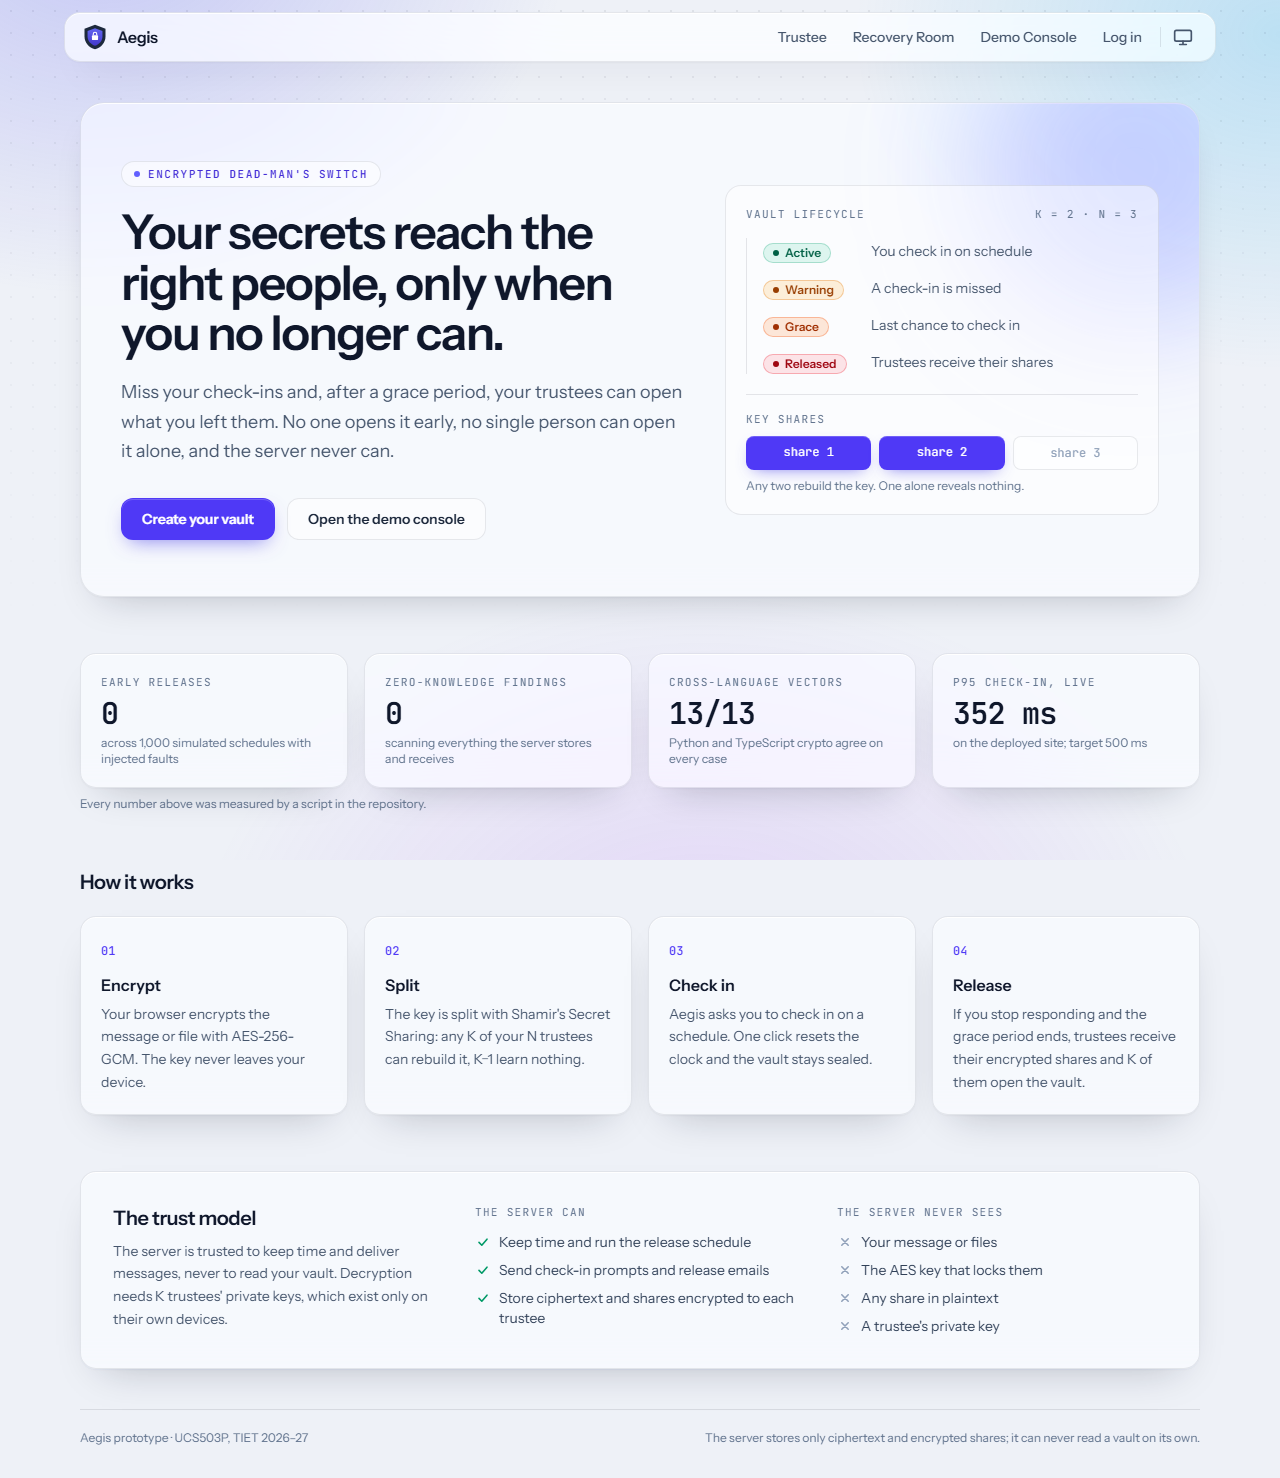
\includegraphics[width=0.92\textwidth,height=0.7\textheight,keepaspectratio]{screenshots/01-landing.png}
  \caption{Landing page: lifecycle and 2-of-3 illustration, measured results and the trust model}
  \label{fig:landing}
\end{figure}

\begin{figure}[htbp]
  \centering
  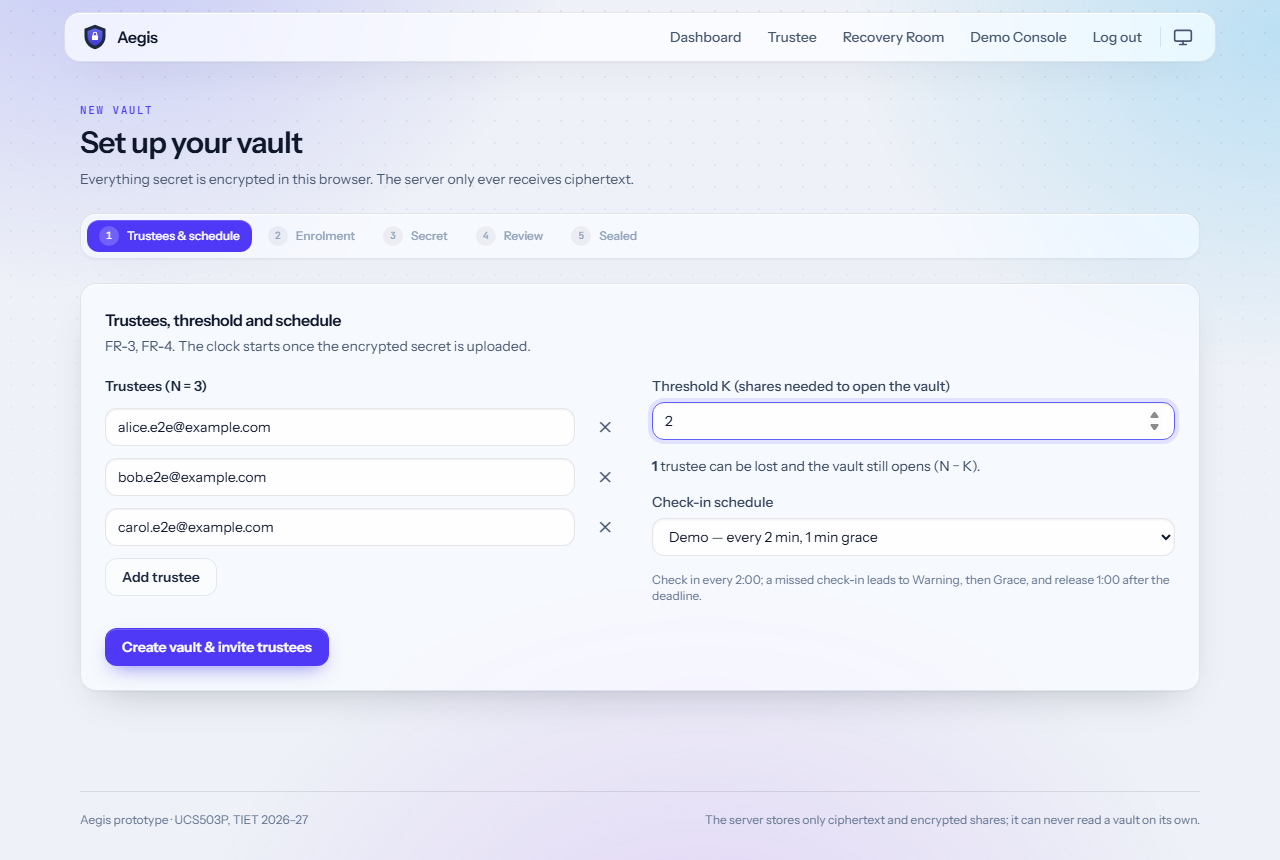
\includegraphics[width=0.92\textwidth,height=0.7\textheight,keepaspectratio]{screenshots/04-wizard-configure.png}
  \caption{Vault wizard: trustees, threshold $K = 2$ of $N = 3$ and loss tolerance}
  \label{fig:wizard}
\end{figure}

\begin{figure}[htbp]
  \centering
  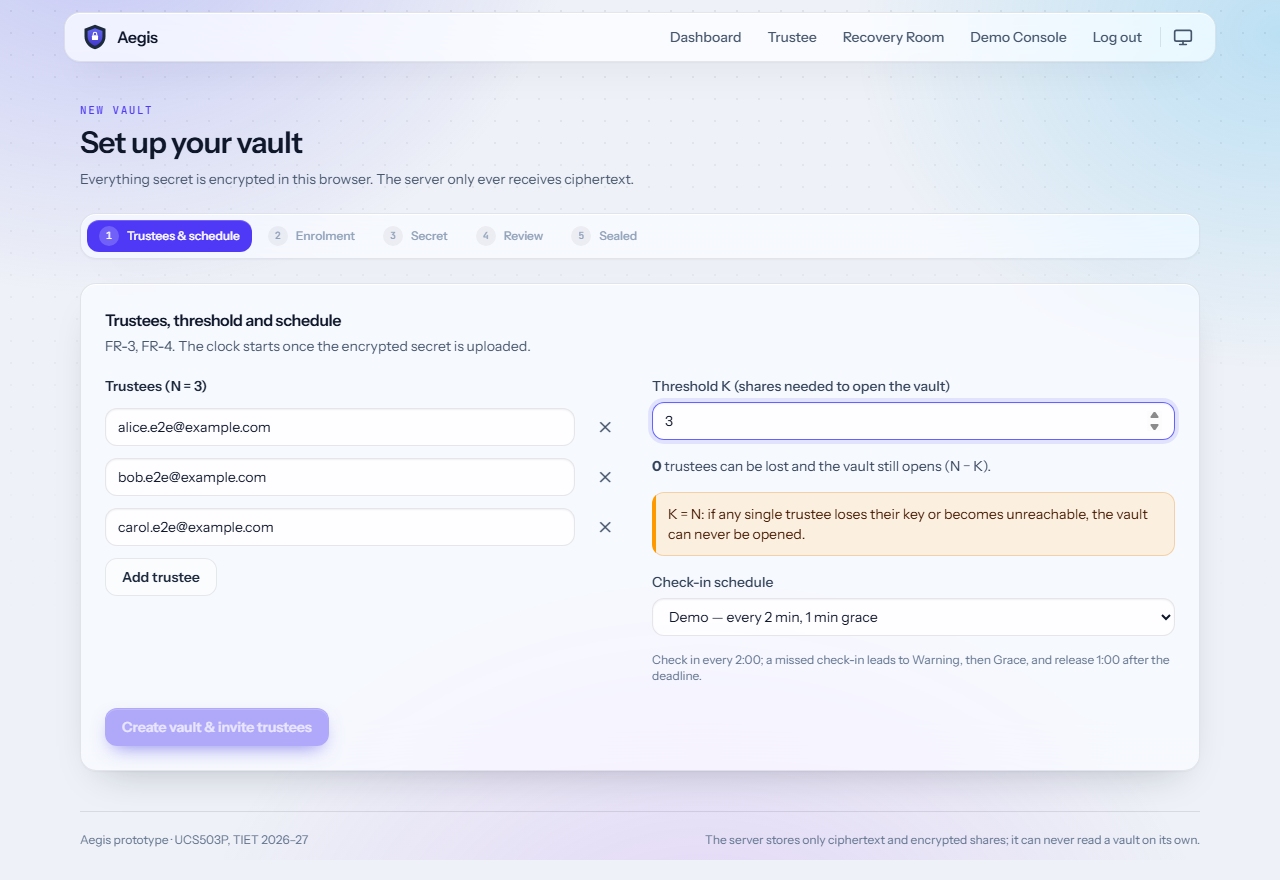
\includegraphics[width=0.92\textwidth,height=0.7\textheight,keepaspectratio]{screenshots/03-threshold-validation.png}
  \caption{FR-4 validation: $K = N$ produces a warning ($K < 2$ is rejected)}
  \label{fig:validation}
\end{figure}

\begin{figure}[htbp]
  \centering
  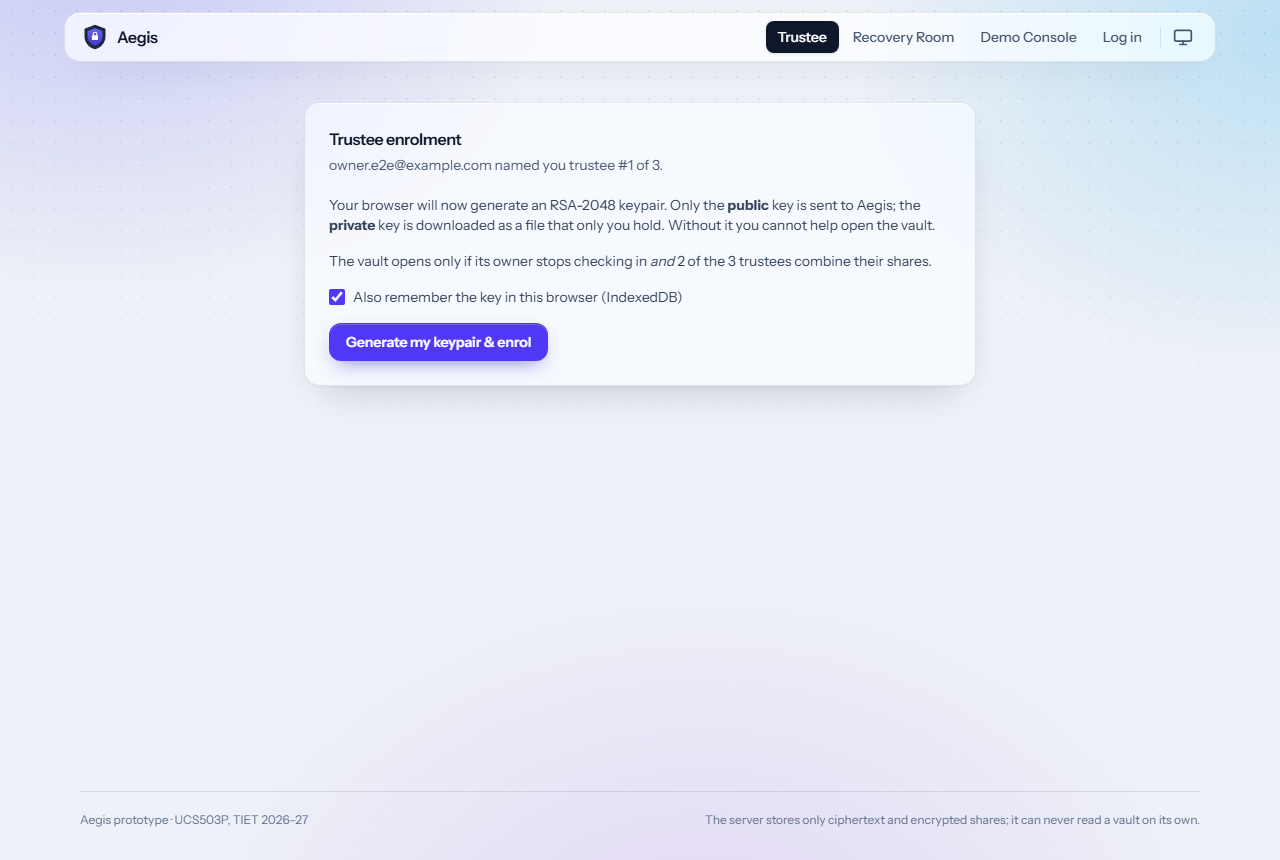
\includegraphics[width=0.92\textwidth,height=0.7\textheight,keepaspectratio]{screenshots/06-trustee-enrol.png}
  \caption{Trustee enrolment: the keypair is generated in the trustee's browser}
  \label{fig:enrol}
\end{figure}

\begin{figure}[htbp]
  \centering
  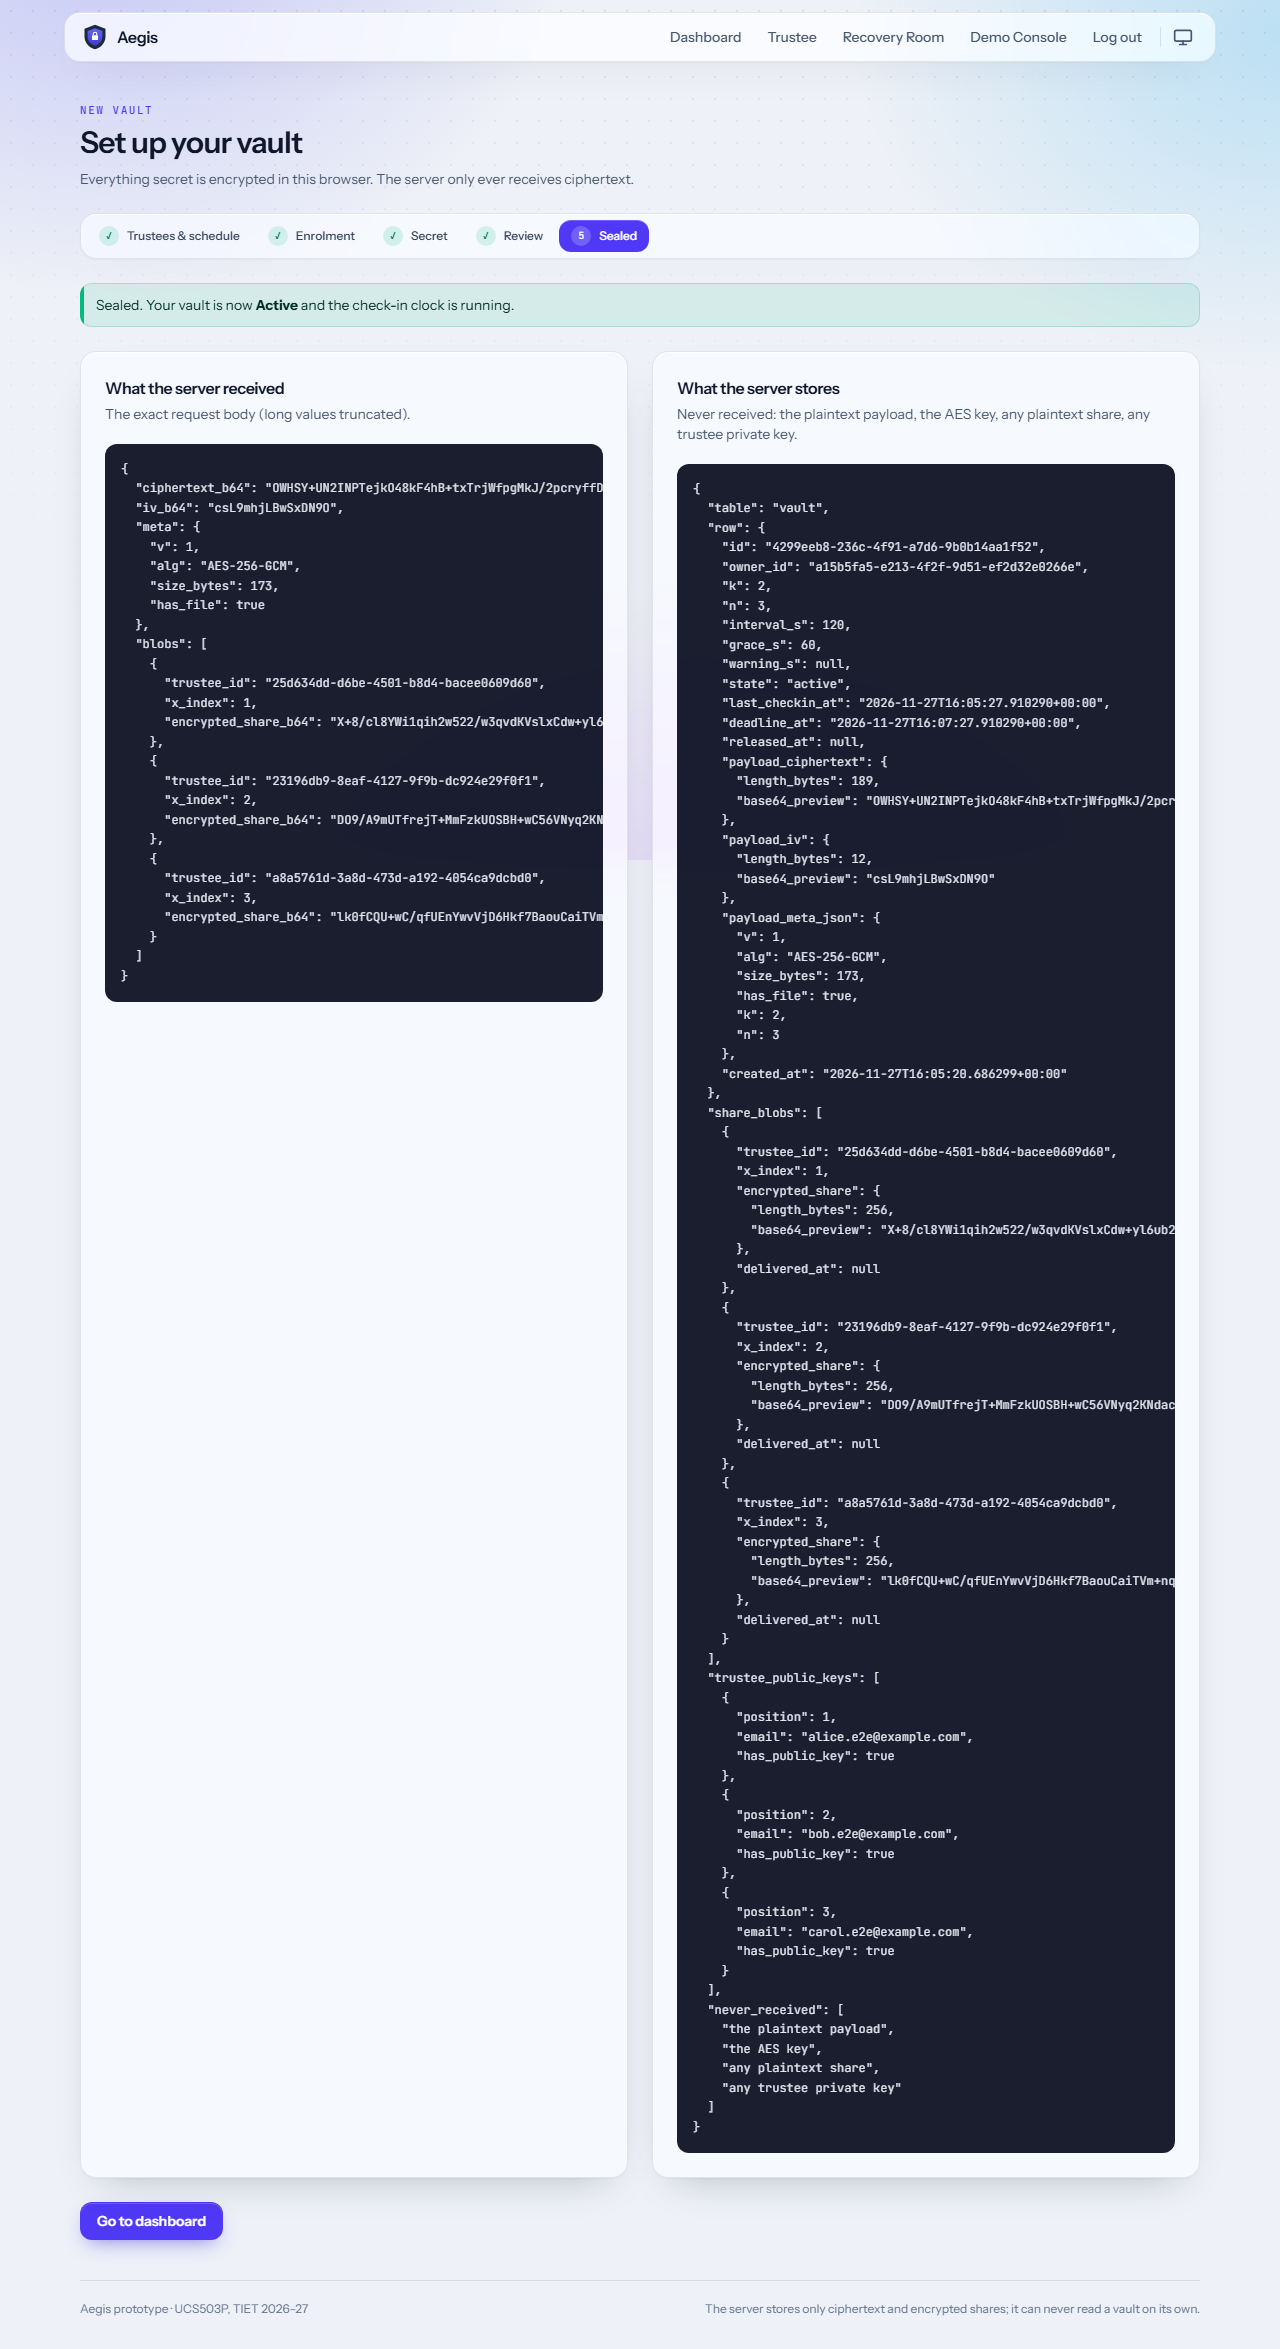
\includegraphics[height=0.72\textheight,width=\textwidth,keepaspectratio]{screenshots/09-server-received.png}
  \caption{What the server received and stores: ciphertext and encrypted shares only}
  \label{fig:server-view}
\end{figure}

\begin{figure}[htbp]
  \centering
  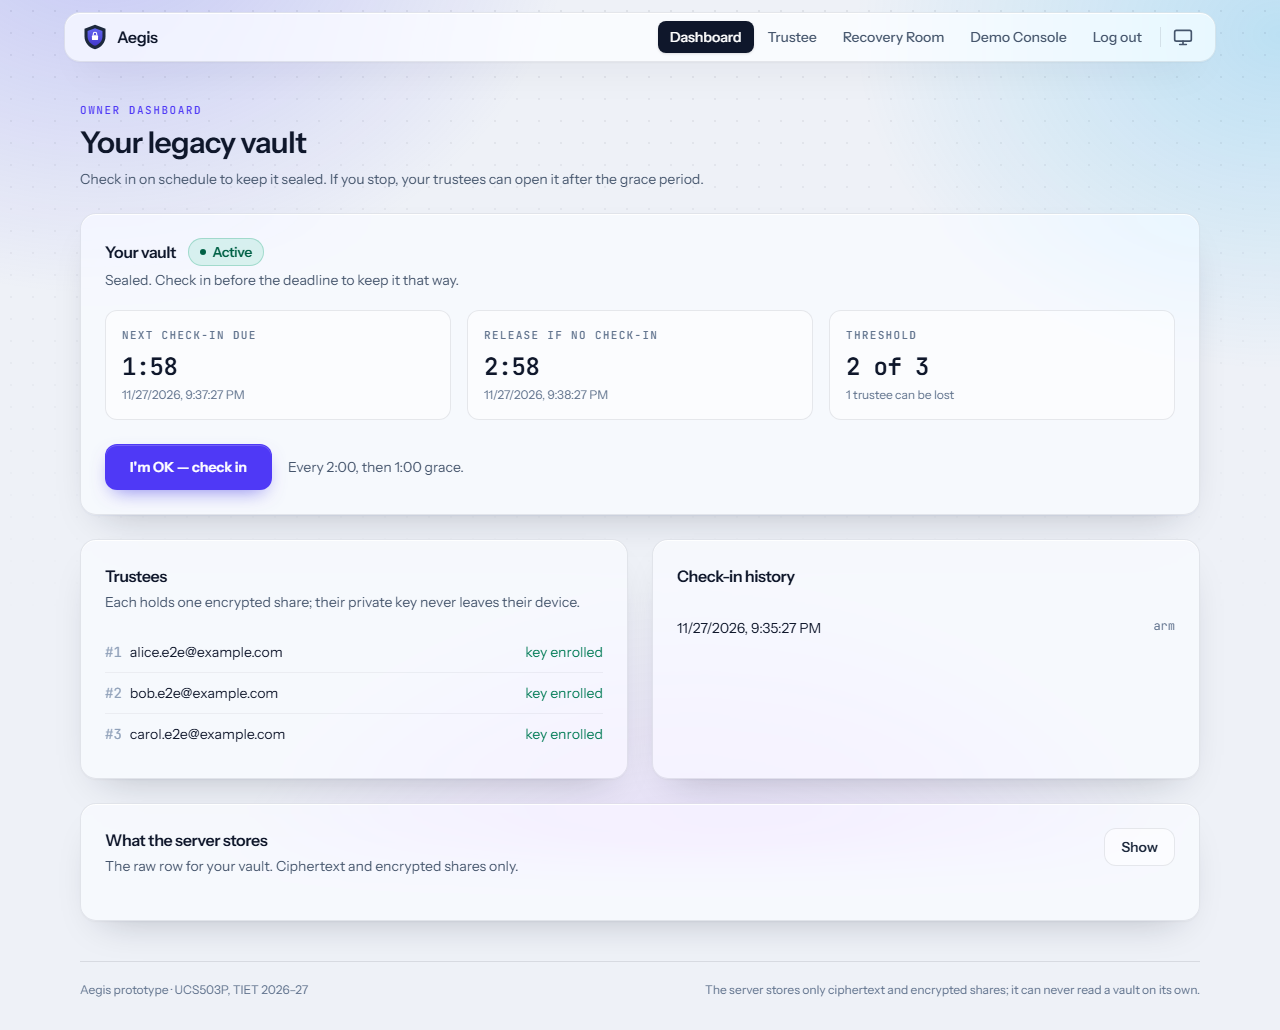
\includegraphics[width=0.92\textwidth,height=0.7\textheight,keepaspectratio]{screenshots/10-dashboard-active.png}
  \caption{Owner dashboard: Active state, live countdowns and one-click check-in}
  \label{fig:dashboard}
\end{figure}

\begin{figure}[htbp]
  \centering
  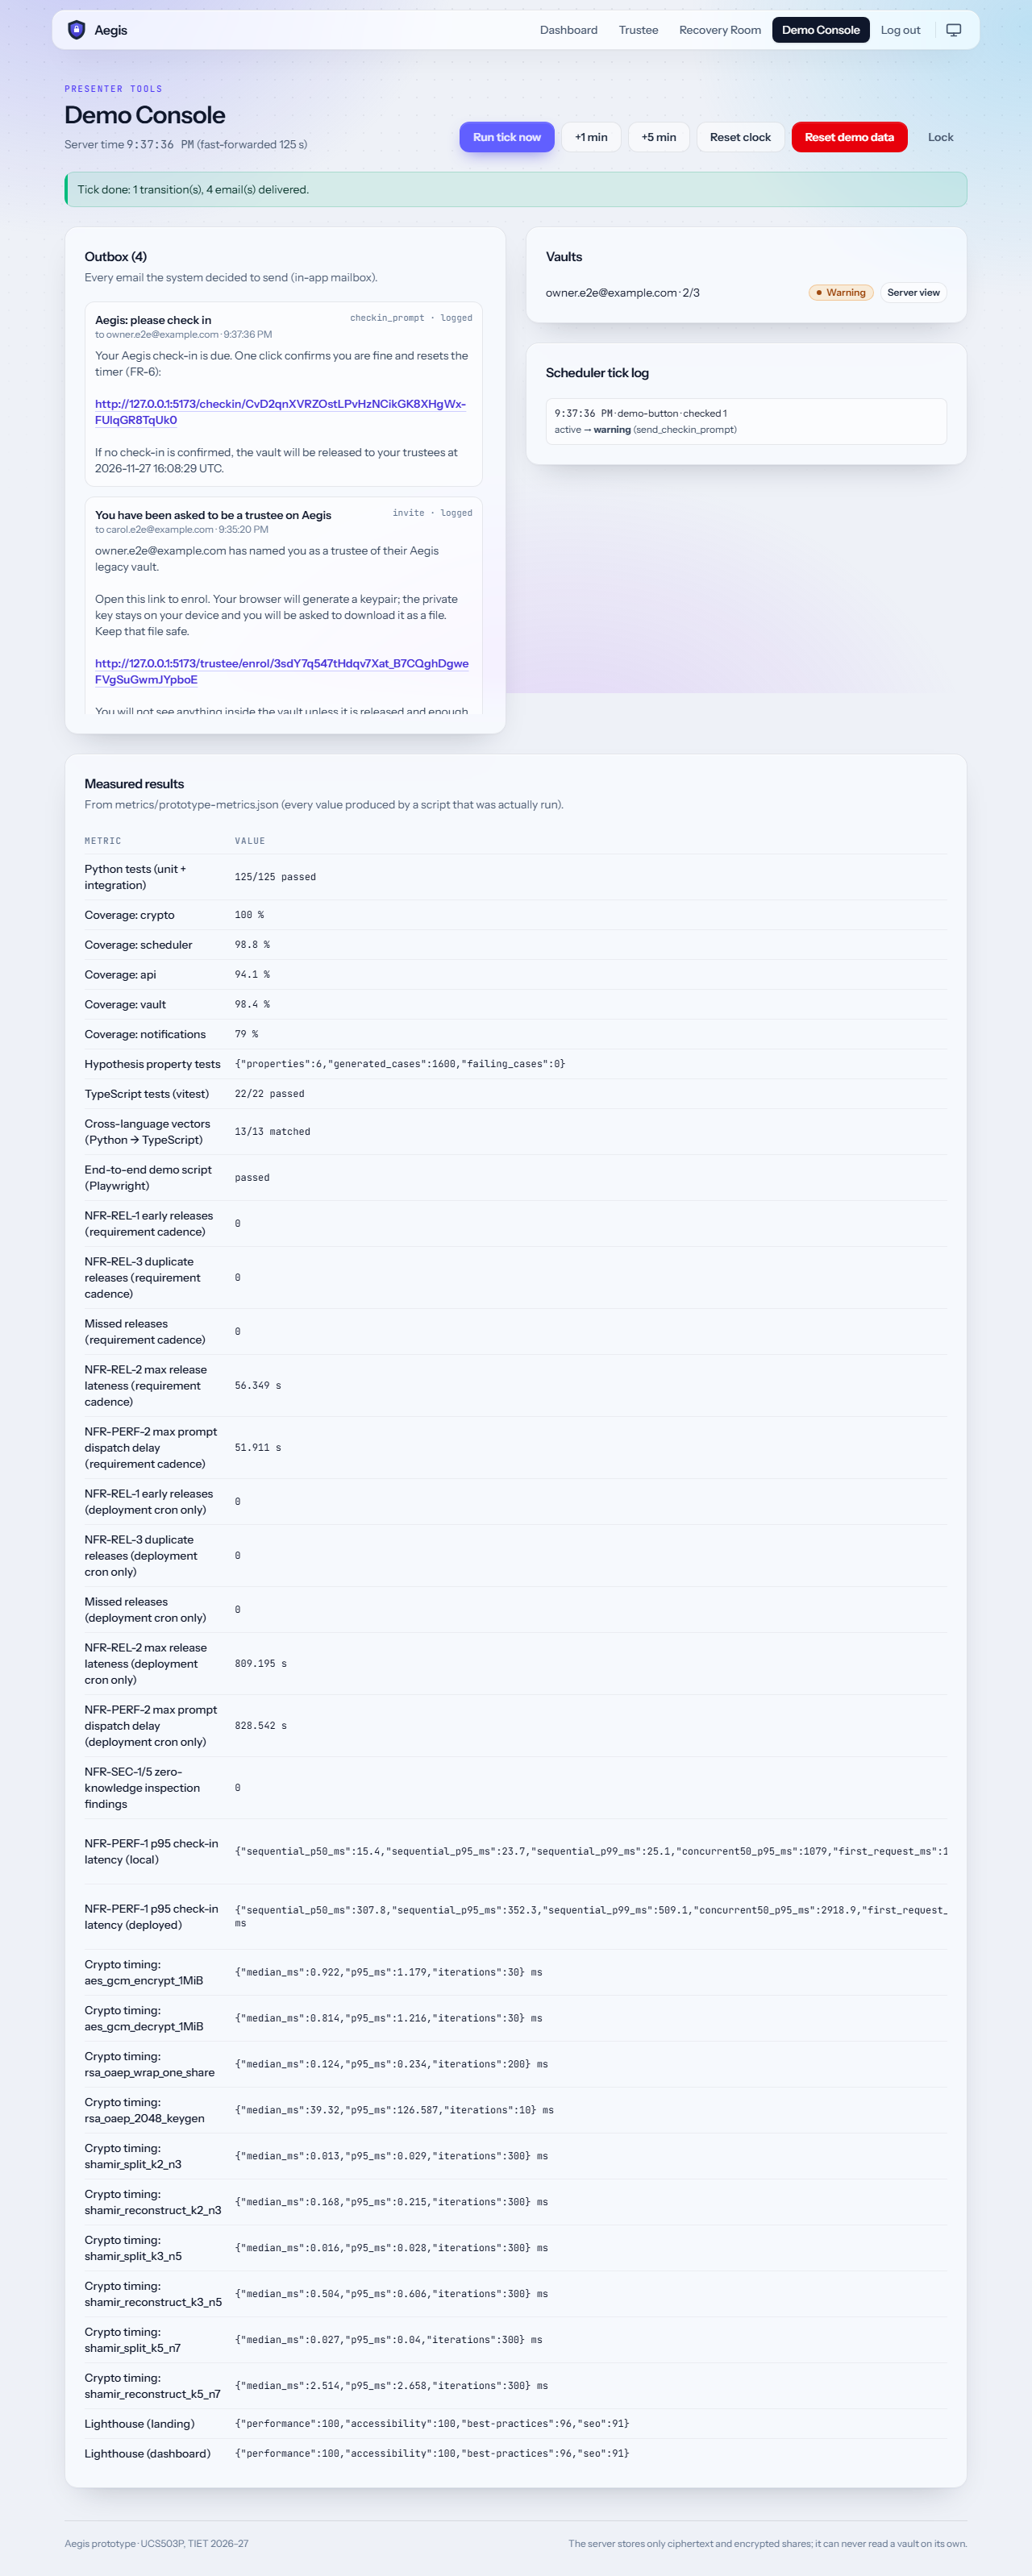
\includegraphics[width=0.92\textwidth,height=0.7\textheight,keepaspectratio]{screenshots/12-demo-console-warning.png}
  \caption{Demo Console after a tick: Warning state and the check-in prompt in the Outbox}
  \label{fig:demo-warning}
\end{figure}

\begin{figure}[htbp]
  \centering
  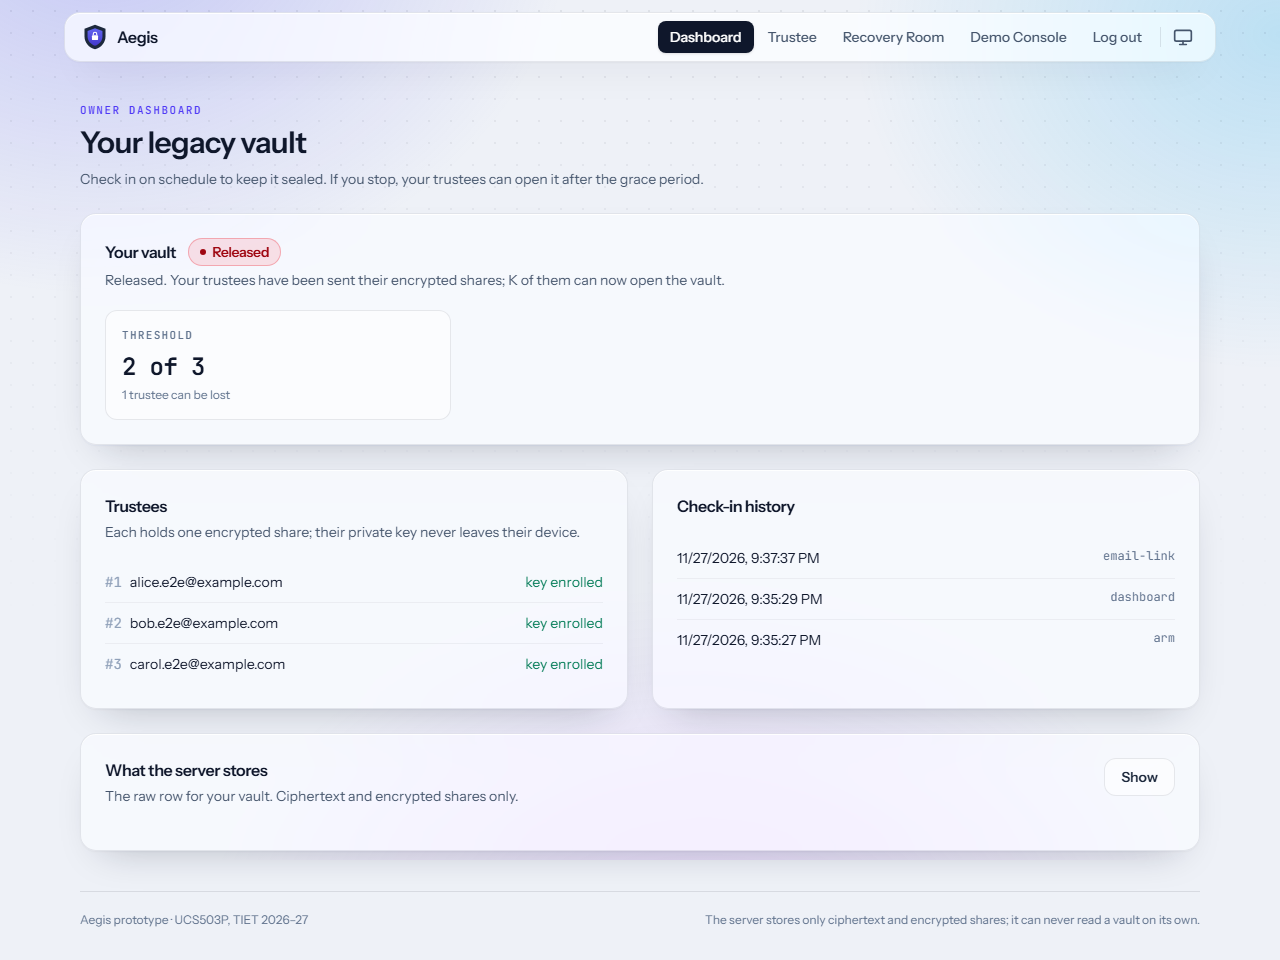
\includegraphics[width=0.92\textwidth,height=0.7\textheight,keepaspectratio]{screenshots/16-dashboard-released.png}
  \caption{The vault after the grace period expired: Released}
  \label{fig:released}
\end{figure}

\begin{figure}[htbp]
  \centering
  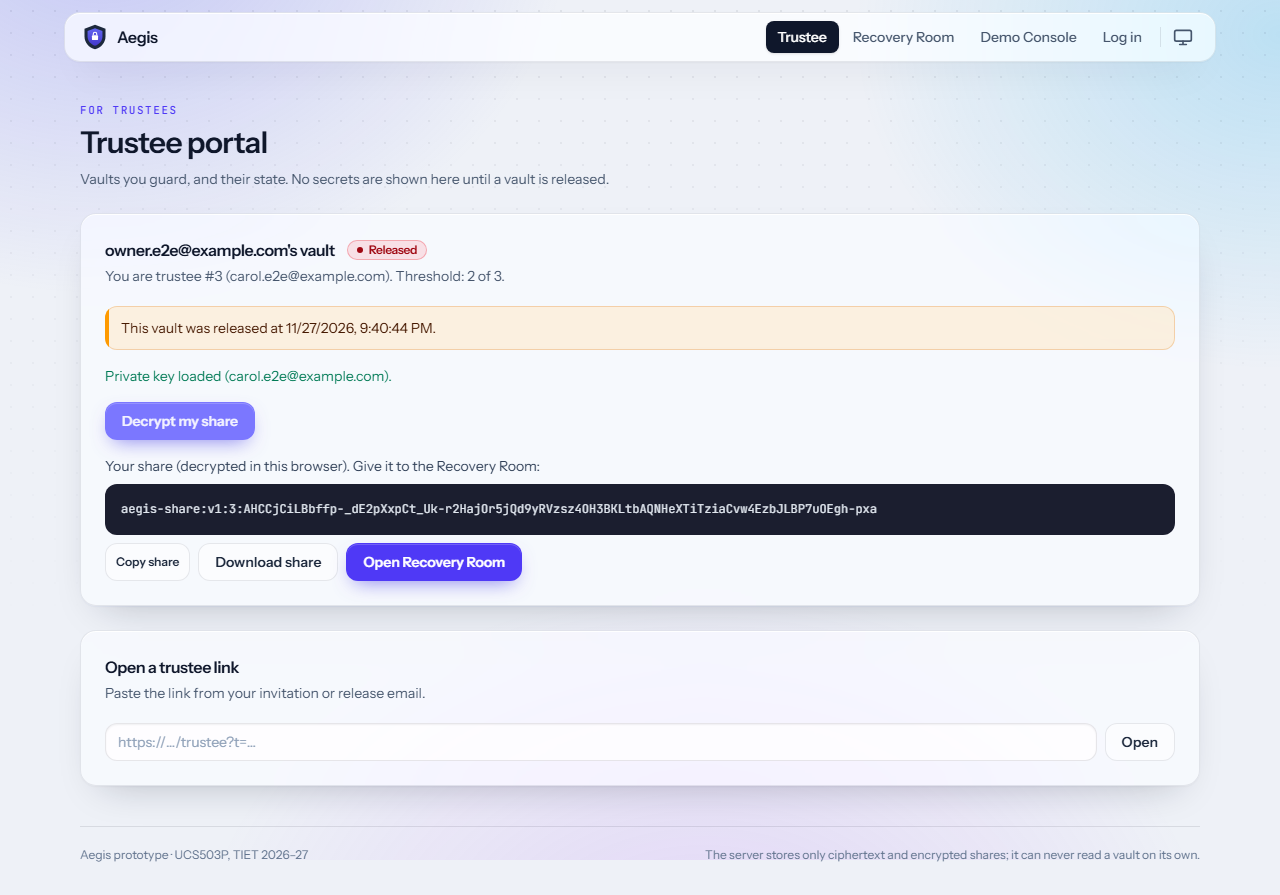
\includegraphics[width=0.92\textwidth,height=0.7\textheight,keepaspectratio]{screenshots/18-trustee-key-file-share.png}
  \caption{Trustee portal: share decrypted in the browser with the private key file}
  \label{fig:trustee-share}
\end{figure}

\begin{figure}[htbp]
  \centering
  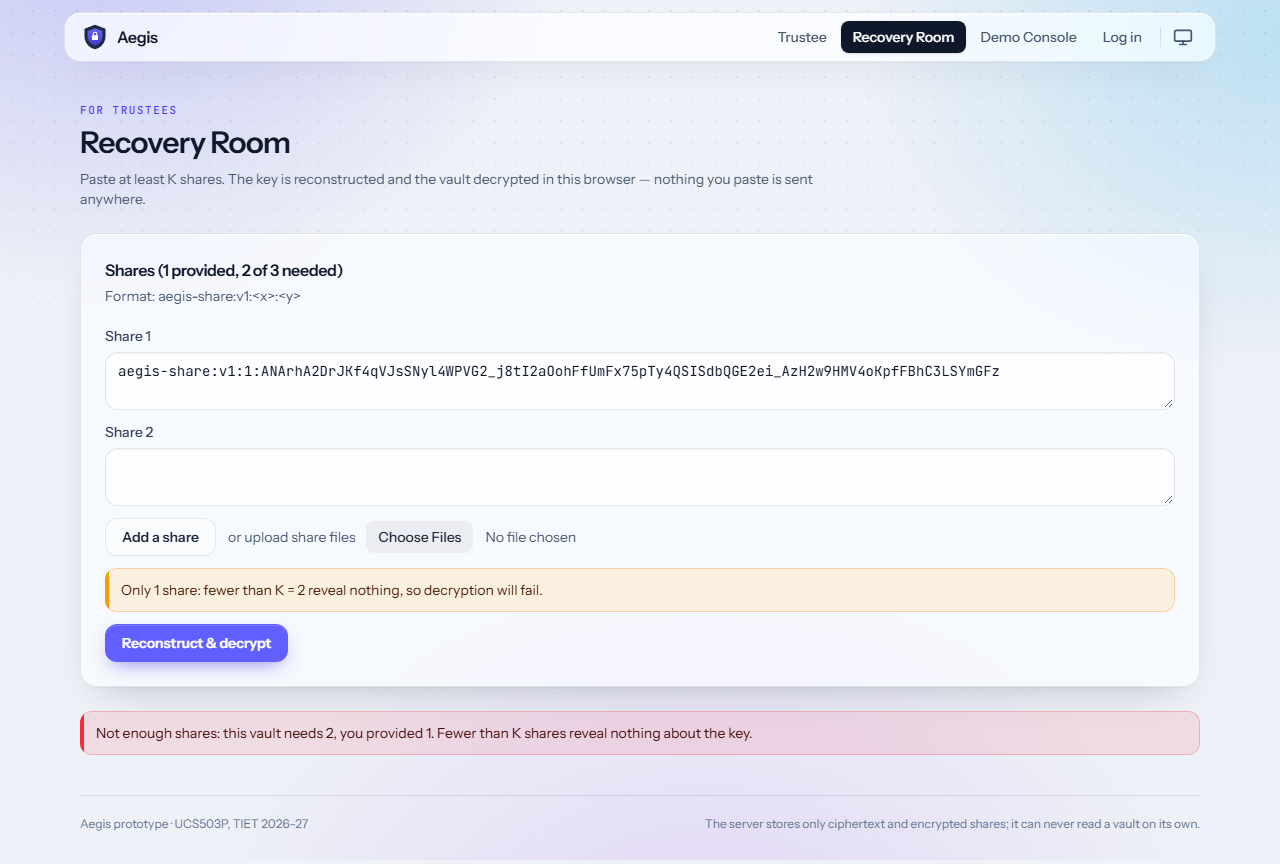
\includegraphics[width=0.92\textwidth,height=0.7\textheight,keepaspectratio]{screenshots/19-recovery-one-share-fails.png}
  \caption{Recovery Room: one share alone is refused}
  \label{fig:one-share}
\end{figure}

\begin{figure}[htbp]
  \centering
  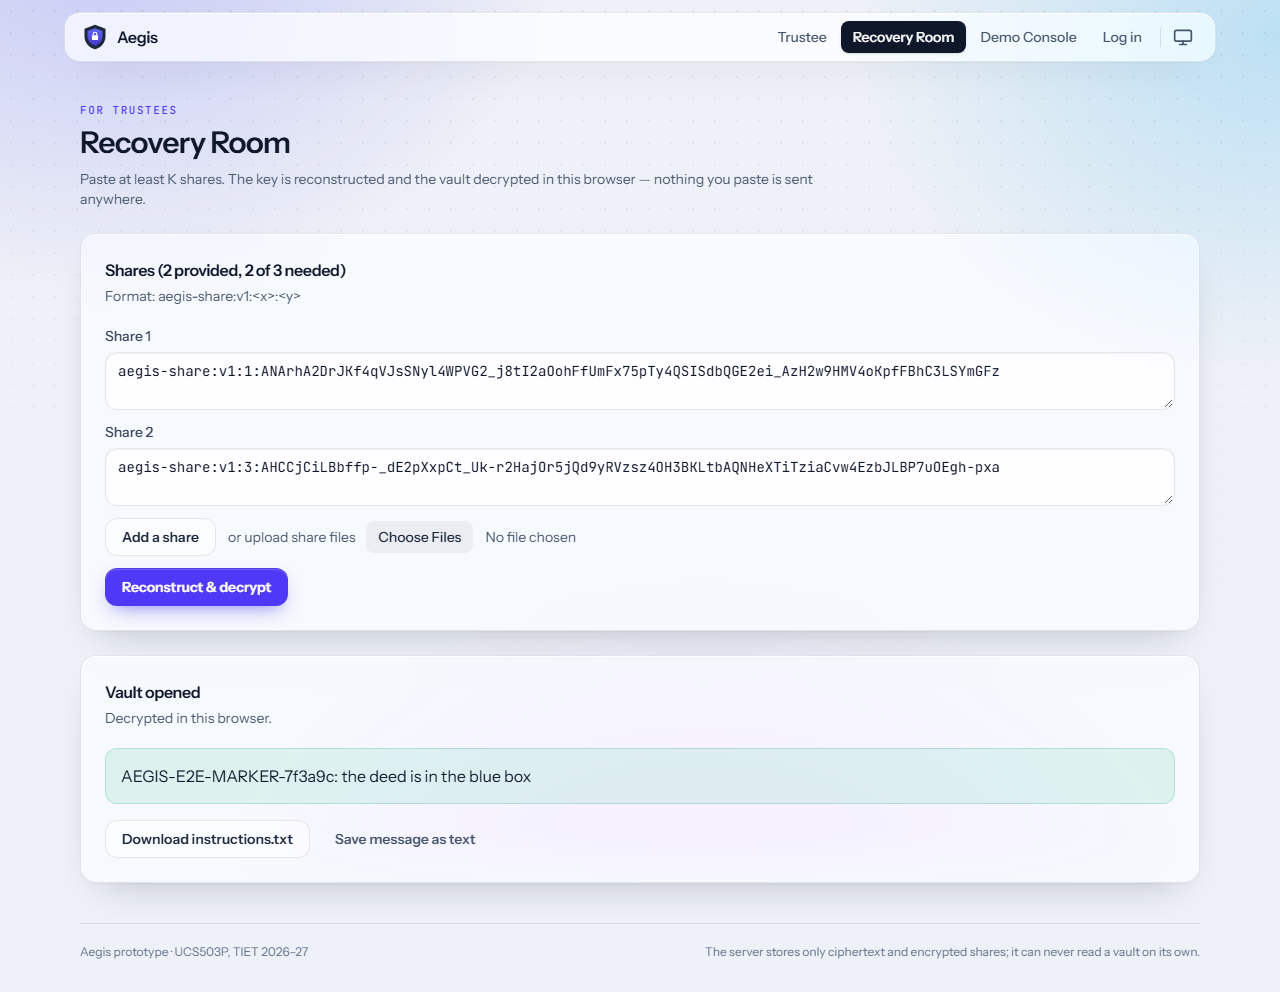
\includegraphics[width=0.92\textwidth,height=0.7\textheight,keepaspectratio]{screenshots/20-recovery-success.png}
  \caption{Recovery Room: two of three shares reconstruct the key and decrypt the vault}
  \label{fig:recovered}
\end{figure}

\begin{figure}[htbp]
  \centering
  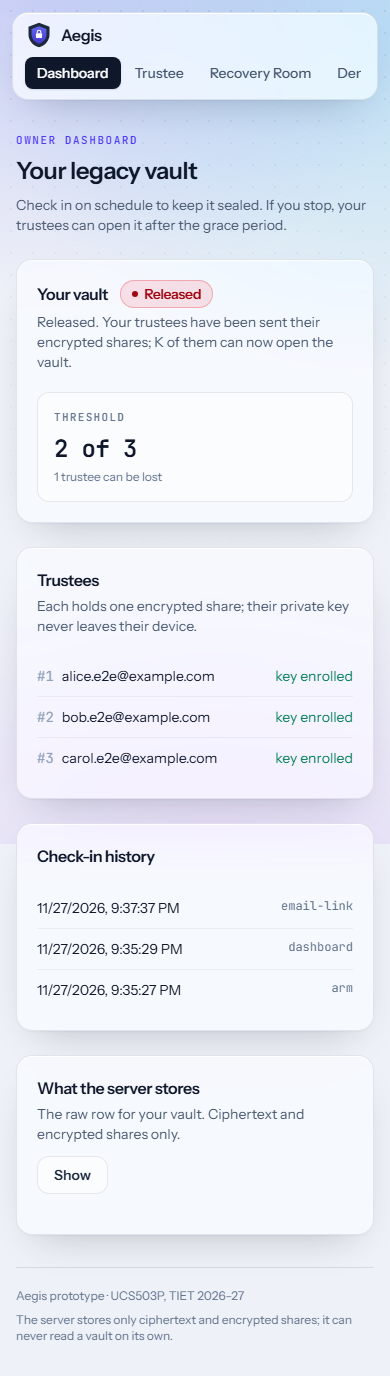
\includegraphics[height=0.6\textheight,width=\textwidth,keepaspectratio]{screenshots/22-dashboard-mobile.png}
  \caption{The dashboard on a phone-sized screen}
  \label{fig:mobile}
\end{figure}

\FloatBarrier

\section{Analysis}\label{sec:results-analysis}

\paragraph{Did we meet our objectives?} Yes for four of the five, and the
fifth is met for its stated nominal load (Table~\ref{tab:objectives}). The
central safety objective was met: across 1,000 simulated schedules with
restarts, racing and duplicate ticks and clock jitter, there were 0 early
releases, 0 duplicate releases and 0 missed releases, and the same held with
the slower deployment cadence. The zero-knowledge inspection found 0
occurrences of the plaintext, the key or any share in the stored data or the
requests, including the database left by the real browser test. The threshold
property was demonstrated end to end in the browser. Coverage on the crypto
and scheduler packages (100.0\% and 98.8\%) exceeds the 80\% target.

\begin{table}[htbp]
  \centering
  \footnotesize
  \caption{Objective status at the final evaluation}
  \label{tab:objectives}
  \begin{tabularx}{\textwidth}{|L{3.2cm}|Y|c|}
    \hline
    \textbf{Objective} & \textbf{Evidence} & \textbf{Status} \\ \hline
    1. Never release early & 0 early, 0 duplicate and 0 missed releases over 1,000 fault-injected schedules & Met \\ \hline
    2. Zero-knowledge server & 0 findings in the automated store and request inspection & Met \\ \hline
    3. Threshold property & 6 Hypothesis properties (1600 cases); end-to-end test: one share refused, two of three recover & Met \\ \hline
    4. Two implementations & 13/13 cross-language vectors matched, enforced in CI & Met \\ \hline
    5. Fast and maintainable, live & Live sequential p95 352.3\,ms; coverage 100.0\% and 98.8\%; 50 simultaneous check-ins on one vault exceed 500\,ms & Met (nominal load) \\ \hline
  \end{tabularx}
\end{table}

\paragraph{Where did we exceed expectations?} Beyond the plan, the Python and
TypeScript implementations were bound by shared known-answer vectors (13/13
matched), the scanner used for the zero-knowledge check carries its own
positive-control self-test, and the whole demo script runs as an automated
test, which also verified the final interface redesign without changes to the
test. Locally, the sequential check-in p95 of 23.7\,ms is well inside the
500\,ms target, and on the live Vercel + Neon deployment it was 352.3\,ms.
Lighthouse scored SEO 100 and Performance 98--100 on the live pages after the
redesign.

\paragraph{What challenges did we encounter, and which targets were missed?}
\begin{itemize}
  \item \textbf{Serverless scheduling.} Vercel functions keep no process alive
    and Hobby-plan cron jobs run at most daily, so the planned APScheduler
    design was replaced by an external trigger. With the 5-minute GitHub
    Actions trigger alone, the maximum release lateness was 809.195\,s and the
    maximum prompt delay 828.542\,s, so \req{NFR-REL-2} and \req{NFR-PERF-2}
    (both 60\,s) are not met by the cron alone. They are met at a cadence of
    under a minute, which the lazy due-checks and the Demo Console provide
    during use and demonstration.
  \item \textbf{Best-effort cron.} GitHub runs scheduled workflows on a
    best-effort basis and delays them under load; on this repository,
    consecutive scheduled runs of the 5-minute workflow were observed hours
    apart, so the cron-only lateness figures above are a lower bound for the
    live site.
  \item \textbf{Email domain.} Without a verified sending domain, Resend
    delivers only to the account owner's address; the in-app Outbox
    (\code{EMAIL\_MODE=log}) keeps the demonstration independent of email
    delivery.
  \item \textbf{Payload size.} Request bodies to Vercel functions are limited,
    so payloads are capped at about 1\,MB and stored in the database; object
    storage for large files is future work.
  \item \textbf{Concurrency.} The load test exposed a stall: FastAPI runs a
    synchronous dependency's setup, the endpoint and the commit as separate
    thread-pool steps, so threads waiting for a database lock could starve the
    lock holder. 50 simultaneous check-ins on one vault still took 1079.0\,ms
    locally and 2918.9\,ms live at the 95th percentile, because writes to one
    vault row are serialised.
  \item \textbf{Glass and readability.} Translucent surfaces make text
    contrast depend on what lies behind a panel. The design therefore uses
    opaque fallbacks, strong surface tints and a contrast check by Lighthouse,
    which found and fixed one failing label.
  \item \textbf{Remaining Lighthouse deductions} are minor: the console logs
    the expected 401 from the logged-out session check (Best Practices 96).
  \item \textbf{Residual security risks} from the threat model remain: a
    malicious operator could serve altered client code (\req{T-4}) or withhold
    a release (\req{T-7}); $K$ or more colluding trustees can open a vault by
    design (\req{T-2}); metadata such as trustee emails and schedules is not
    encrypted; and one moderate advisory remains in React Router~6.
\end{itemize}

\paragraph{How did we resolve them?} The scheduler was redesigned around a
pure decision function and an idempotent, transactional tick with several
independent triggers; exactly-once delivery is enforced by unique
deduplication keys in the outbox; the thread-pool stall was removed by
limiting in-flight requests below the pool size; an invalid package name
inherited from the course template, which broke Vercel's dependency
installation, was corrected; and the redesign kept every interface element the
end-to-end test relies on, so it could be verified automatically. Each fix was
confirmed by re-running the relevant measurement.

% ===== CHAPTER 4: CONCLUSION =====

\chapter{Conclusion}\label{ch:conclusion}

\section{Summary of Work}\label{sec:conclusion-summary}

The team built and deployed Aegis, an encrypted dead-man's-switch vault in
which the browser encrypts a secret, splits its key with Shamir's Secret
Sharing and wraps each share for a trustee, and the server only keeps time and
stores ciphertext. The final product covers the full demonstration script ---
registration, trustee enrolment with browser-generated keys, sealing,
one-click check-in, the Active, Warning, Grace and Released lifecycle, share
decryption by trustees and $K$-of-$N$ recovery --- runs live on Vercel with
Neon Postgres, and has a redesigned interface with light and dark themes. It
is accompanied by a measurement suite whose results are reported in
Chapter~\ref{ch:results}. Objectives 1--4 were met in full and Objective 5 for
its nominal load.

\section{Key Findings}\label{sec:conclusion-findings}

\begin{itemize}
  \item \textbf{Finding 1:} A pure decision function plus a transactional,
    idempotent tick made the never-early and exactly-once properties testable
    at scale: 0 early and 0 duplicate releases over 1,000 fault-injected
    schedules.
  \item \textbf{Finding 2:} A zero-knowledge server is practical with standard
    browser cryptography: the inspection found 0 secrets on the server, and
    client-side costs are small (AES-256-GCM over 1\,MiB in a median of
    0.922\,ms).
  \item \textbf{Finding 3:} On serverless hosting, timeliness depends on the
    tick trigger rather than on the code: the same scheduler meets the
    60-second targets at a sub-minute cadence but not with a 5-minute cron
    alone.
  \item \textbf{Finding 4:} Treating the demonstration as an automated test
    paid off at the end of the project: the whole interface was redesigned in
    one change and verified by the same end-to-end script, with no change to
    the test.
\end{itemize}

\section{Future Work and Recommendations}\label{sec:conclusion-future}

\begin{enumerate}
  \item \textbf{Enhancements:} multiple vaults per owner, editing a vault
    after creation, account recovery, two-factor authentication, trustee-side
    reminders and an audit export.
  \item \textbf{Alternative approaches:} verifiable secret sharing so that
    tampered shares are rejected (threat \req{T-9}), constant-time field
    arithmetic, and a signed or extension-delivered client to remove the
    code-delivery risk (threat \req{T-4}).
  \item \textbf{Scalability:} object storage for files larger than 1\,MB,
    Alembic migrations, rate limiting and a dedicated scheduler (or a paid
    cron) to meet \req{NFR-REL-2} without relying on lazy due-checks.
  \item \textbf{Integration:} a production email domain with Resend, and
    optional notification channels behind the existing \code{EmailSender}
    strategy (SMS remains out of scope under \req{NG-1}).
  \item \textbf{Real-world deployment:} an independent security review, the
    upgrade to React Router~7, an admin interface, monitoring of the tick
    triggers, usability testing with people outside the team, and backup and
    retention policies for the encrypted store.
\end{enumerate}

\section{Final Remarks}\label{sec:conclusion-remarks}

Building Aegis taught us to treat the demonstration as an acceptance test:
once the five-minute demo script ran as an automated browser test, every
change --- including the final redesign --- was checked against what we would
actually present. We also learned to measure rather than estimate. Every number
in this report comes from a script in the repository, including the two
timeliness targets that the cron trigger alone does not meet and the
accessibility issue that re-measurement uncovered. Finally, serverless hosting
changed the design more than we expected: with no long-running process, the
scheduler became a pure function triggered from outside, which turned out to
be easier to test and to reason about.

% ===== BIBLIOGRAPHY =====

% Print bibliography with heading in TOC
\printbibliography[heading=bibintoc]

\end{document}
